\documentclass[12pt,letterpaper,ngerman]{article}
%\usepackage[letterpaper,top=3.0cm, bottom=3.0cm, footnotesep=1.0cm]{geometry}
\usepackage[letterpaper,margin=1in]{geometry} % e. Set margins of 1 inch (2.54 cm.) on all four sides of the paper. 
\usepackage{mathptmx} % d. ...in a simple roman face except where indicated below (§3). 
\usepackage[singlespacing]{setspace} % Set line spacing to 1 throughout the document
\usepackage{fancyhdr} 

% Set the headheight to at least 14.49998pt
\setlength{\headheight}{14.49998pt}

% Optionally adjust \topmargin if necessary
% \addtolength{\topmargin}{-2.49998pt}
\usepackage{relsize}

\usepackage[bottom]{footmisc}
\usepackage{tabularx}
    
\pagestyle{empty}        % No page numbers

% Set paragraph indentation to 1.5cm
\setlength{\parindent}{2em}

%%%Using XeTeX (xelatex, lulatex):
%\usepackage{polyglossia}
%\usepackage{fontspec}
%\usepackage{xunicode}
%\usepackage{xltxtra}
\usepackage{url}
\usepackage{hyperref}
\usepackage[english,german]{babel}

\usepackage{graphicx}

%\setmainfont[Mapping=tex-text]{Linux Libertine O} %Falls nicht vorhanden müssen die LinLibertine-ttf-Dateien nach C:\windows\fonts verschoben werden

\usepackage{booktabs}    % For nice-looking tables
\usepackage{natbib}      % Citation support (required for crossrefs)
\usepackage{expex}
\bibpunct[:]{(}{)}{;}{a}{}{,} % Defaults for in-text citations
\usepackage{bibentry}    % Print individual references

\usepackage{acronym}
\usepackage{multicol}

% TODO: set authors name
%vorgelegt von\\
%Name des Verfassers/der Verfasserin\\
\author{Author's name}

\usepackage{scrhack} % Recommended to avoid potential conflicts
\usepackage{microtype}

\usepackage[acronym,xindy,toc]{glossaries} % TODO: include "acronym" if glossary and acronym should be separated
\makeglossaries
\loadglsentries{pages/glossary.tex} % important update for glossaries, before document

\usepackage{ragged2e}

% Set up hyphenation rules for the language package when mistakes happen
\babelhyphenation[english]{
an-oth-er
ex-am-ple
}

\usepackage{babel}
\usepackage{csquotes}
\usepackage{pgfplots}
\MakeOuterQuote{"}
\usepackage{mathtools}
\usepackage{amssymb}
\usepackage{amsmath}
\usepackage{tikz}
\usepackage{chngcntr}
\usepackage{float}
\usepackage{svg}
\usepackage{cite}
\usepackage{bookmark}
\usetikzlibrary{
  decorations.pathmorphing,
  automata, positioning, arrows, matrix,
  decorations.pathreplacing,
  shapes.geometric, calc,shapes.misc,
  arrows.meta,backgrounds,fit,petri
}
\pgfmathsetseed{\number\pdfrandomseed} % to ensure that it is randomized
\begin{document}
\DeclarePairedDelimiter\ceil{\lceil}{\rceil}
\DeclarePairedDelimiter\floor{\lfloor}{\rfloor}
\newcommand{\rand}[2]{
\pgfmathsetmacro{\thenum}{rand(0,1)}
\thenum
}
\newcommand{\nat}[0]{\mathbf{N}}
\newtheorem{example}{Beispiel}[section]


\begin{center}\uppercase{Ludwig-Maximilians-Universität München}\end{center}
\begin{center}
  \uppercase{Programming languages and artificial intelligence}
\end{center}

\vspace*{10mm}
\begin{center}

\includegraphics[height=40mm]{abb/sigillum.png}
\end{center}
\vspace*{10mm}

\title{Titel der Arbeit}
\date{\vspace{-5ex}}
{\let\newpage\relax\maketitle}
\thispagestyle{empty}
\begin{center}
\begin{large}
\begin{Large}
Bachelorarbeit
\end{Large}
im Studiengang 'Informatik plus Mathematik' 
\end{large}
\end{center}
\vspace{1cm}
\begin{center}
\begin{large}
Betreuer: Prof. Dr. Johannes Kinder
\end{large}
\end{center}
\begin{center}
\begin{large}
Mentor: Moritz Dannehl, M.Sc.
\end{large}
\end{center}


\begin{center}
\begin{large}
Ablieferungstermin: \date{\today} 
\end{large}
\end{center}

\vspace{1,5cm}

\newpage
\tableofcontents
\newpage

\setcounter{page}{1}
\pagestyle{fancy}
\fancyhf{}
\counterwithin{figure}{section}
\fancyhead[R]{\thepage}
\renewcommand{\headrulewidth}{0pt} %obere Trennlinie
\newtheorem{definition}{Definition}
\section*{Abstract}
\section{Einführung}
In den letzten Jahren wurden wichtige Fortschritte in der natürlichen
Sprachverarbeitung erzielt, ein wichtiger Faktor war die Codierung von
natürlicher Sprache in reellwertigen Vektoren (engl. embeddings). Die hochdimensionalen Vektoren
codieren die Semantik der ursprünglichen Wörter oder Sätze. Die daraus 
resultierenden Vektoren erlauben es, neuronale Netzwerke in diversen 
Anwendungsbereichen zu trainieren, wie beispielsweise
\textit{Spam Detection} \cite{Ball2019}.  
Zu den bekanntesten Modellen, die natürliche Sprache in Vektoren abbilden, gehören 
\textit{Word2Vec} \cite{word2vec},
\textit{WordPiece} \cite{wu2016googlesneuralmachinetranslation} und
\textit{SentenceTransformer} \cite{reimers-2019-sentence-bert}. 

Diese Fortschritte dienen als Motivation, auch Assembler Quellcode auf einen 
Vektor abzubilden, der die Semantik des Quellcodes codiert. Die resultierenden
Vektoren können dann wieder benutzt werden, um neuronale Netzwerke auf
diverse Anwendungen zu trainieren, wie beispielsweise
\textit{Binary Code-Similarity-Detection} \cite{jtrans},
\textit{Function-Boundary-Detection} \cite{190918},
\textit{Function-Type-Inference}\cite{203650},
\textit{Binary Code-Search} \cite{9345532},
Reverse Engineering \cite{reverse-engeneering},
oder das Klassifizieren von 
Maleware in der Maschinensprache\cite{maleware-detection}.

Um ein Modell mittels überwachtes Lernen zu trainieren, das Assemblercode in 
semantische Vektoren abbildet, ist für jede Assembler-Funktion ein Vektor 
erforderlich, der die Semantik der Funktion codiert. Der Datensatz kann durch 
Kompilieren des Quellcodes von höheren Programmiersprachen generiert 
werden.

Das Ziel dieser Arbeit ist es, verschiedene Methoden zu vergleichen
aus C Quellcode Vektoren zu generieren, die die Semantik von dem ursprünglichen
Quellcode codieren, mithilfe von Werkzeugen aus der natürlichen Sprachverarbeitung.

Der Prozess des Kompilierens reduziert Funktionen
auf die für den Computer wesentlichsten Bausteine, dabei gehen viele 
Informationen verloren, wie Funktionsnamen, Variablennamen und Kommentare. 
Diese Informationen sind von großer Bedeutung und geben Aufschluss über 
die Funktionsweise und den Anwendungszweck der Funktion. Durch die Verwendung 
dieser Informationen könnte die semantische Codierung des Quellcodes verbessert
werden. Aufgrund der Tatsache, dass diese Informationen in der natürlichen 
Sprache sind, ist es sinnvoll, bewährte Werkzeuge aus der natürlichen 
Sprachverarbeitung zu verwenden, um diese in semantische Vektoren zu codieren. 
Aus den resultierenden Vektoren kann schließlich ein Datensatz generiert werden,
der ein neuronales Netzwerk darauf trainiert, Assemblercode auf hochdimensionale,
reellwertige Vektoren abzubilden, die die Semantik des Quellcodes codieren.
\pagebreak
\subsection{Stand der Technik}
{\bf CLAP} ({\bf C}ontrastive {\bf L}anguage {\bf A}ssembly {\bf P}re-training) 
\cite{clap} 
setze Anfang 2024 einen neuen Stand der Technik, in
\textit{Binary Code-Simillarity-Detection}
mithilfe von natürlicher Sprachverarbeitung. Die Aufgabe bei 
\textit{Binary Code-Simillarity-Detection}
besteht darin, die semantische Ähnlichkeit zwischen zwei gegebenen 
Assemblercodes zu bestimmen.

Das CLAP-Modell ist aus zwei Teilen zusammengesetzt: einem Assembler-Encoder 
und einem Text-Encoder. Der Assembler-Encoder, der aus Assemblercode 
reellwertige Vektoren erzeugt, knüpft mit kleinen Änderungen an den vorherigen
Stand der Technik von JTrans an. Der Text-Encoder ist eine völlig neue Idee, 
die darauf abzielt, den Text wieder in einen reellwertigen Vektor zu 
konvertieren. Wang et al. starten dabei mit einem Modell aus der natürlichen 
Sprachverarbeitung namens \textit{SentenceTransformer} und trainieren dieses
darauf, Assemblercode die passende Quellcodeerklärung  zuzuordnen. Dabei 
erhalten sie die Quellcodeerklärungen durch ein Large  Language-Model, wie
beispielsweise Chat-GPT.

{\bf JTrans} \cite{jtrans}
baut auf einer Modellarchitektur aus der natürlichen 
Sprachverarbeitung namens 
Transformer \cite{transformer} auf. 
Wang et. al behandeln die einzelnen Assembler-Instruktionen als Wörter, um so 
die Transformer-Modellarchitektur anwenden zu können. Außerdem codieren sie
Kontrollflussinformationen des Assembler-Codes in die Eingabe des 
Transformer-Modells. Mit diesem Ansatz erzielten sie im Jahre 2022 einen neuen
Stand der Technik in \textit{Binary Code Similarity Detection}.

\subsection{Leistungen der Arbeit}
Die hauptsächlichen Leistungen dieser Arbeit sind:
\begin{itemize}
  \item ein Tool, das einen Datensatz mit Assemblercode und semantischen 
    Vektoren aus C-Quellcode und dem dazugehörigen Assemblercode generiert.
  \item eine qualitative Analyse durch 
    \textit{t-SNE} \cite{JMLR:v9:vandermaaten08a}, die die Verwendung von 
    Funktionskommentaren, Funktionsnamen, 
    \textit{Code Llama} \cite{rozière2024codellamaopenfoundation} Erklärungen
    und  \textit{Code2Vec}  \cite{code2vec}
    untersucht.
  \item eine quantitative Auswertung, die durch Befragung von Experten erfolgt,
    vergleicht die Verwendung von Funktionsnamen, \textit{Code Llama} 
    Erklärungen und  \textit{Code2Vec}  miteinander.
  \item eine Formel, die die Verwendung von Funktionsnamen, \textit{Code Llama}
    Erklärungen und  \textit{Code2Vec}  vergleicht.
\end{itemize}
\pagebreak
\subsection{Aufbau der Arbeit}
Kapitel 2 führt anfangs grundlegende Konzepte und Begriffe des maschinellen 
Lernens ein. Anschließend werden semantische Vektorräume in Bezug auf 
natürliche Sprache erläutert und die größten Fortschritte der letzten Jahre 
beschrieben. Am Ende werden noch \textit{Code Llama},  \textit{Code2Vec}  und 
\textit{t-SNE} vorgestellt, welche eine wichtige Rolle in dieser Arbeit spielen.

Die allgemeine Architektur des Tools und dessen Designentscheidungen werden im Kapitel 3
beschrieben. Es werden die Auswahl des C-Quellcodes, die Datenpipeline und die 
Stabilität des \textit{SentenceTransformers} erläutert.

Kapitel 4, 5, 6 und 7 befassen sich mit den verschiedenen Methoden, Embeddings
zu erzeugen. Also wie aus den Quellcodeinformationen über Funktionsnamen und
-kommentare ein Vektor erstellt werden kann. Außerdem wird erläutert, wie mit
\textit{Code Llama} und  \textit{Code2Vec}  Vektoren produziert werden können.

Die Ergebnisse werden in einer qualitativen und quantitativen Auswertung in 
Kapitel 8 vorgestellt. Zuerst wird durch eine Experten-Evaluierung die beste
Methode identifiziert. Anhand dieser Einordnung wird überprüft, ob die Formel
und Analyse durch \textit{t-SNE} ein ähnliches Ergebnis aufweisen.

Die Ergebnisse werden im Kapitel 9 reflektiert, eingeordnet und diskutiert. 
Es werden die Stärken und Schwächen jeder Methode dargestellt und diskutiert.

Im letzten Kapitel wird die gesamte Arbeit reflektiert und anschließend ein 
Ausblick gegeben, um weitere Anregungen für die weitere Arbeit in diesem Thema
zu geben.

\pagebreak
\section{Grundlagen}
\subsection{Maschinelles Lernen}
Heutzutage ist maschinelles Lernen weitverbreitet und wird in nahezu jedem
Bereich der Informatik verwendet.  Maschinelles Lernen wird überall dort 
eingesetzt, wo eine analytische Lösung eines Problems zu aufwendig oder gar 
überhaupt nicht existiert. Maschinelles Lernen sucht nach einer Lösung, indem 
es aus den Daten ein Muster ableitet. Sind die Daten endlich, ist meist das 
resultierende Modell nur eine Approximation der gesuchten Lösung. In diesem 
Abschnitt wird zunächst maschinelles Lernen definiert und dann darauf aufbauend 
grundlegende Trainingsarten vorgestellt.
 % Book: Learingin from data, page 1, row 6
\subsubsection{Definition}
Die weit verbreitete Ansicht, dass maschinelles Lernen nur etwas mit neuronalen 
Netzwerken zu tun hat, ist im Allgemeinen falsch. Generell kann ein Problem, 
das mit maschinellem Lernen gelöst wird, wie folgt definiert werden:
\begin{definition}
  Sei $X$ eine beliebige Input Menge, $Y$ eine beliebige Output Menge,
  $f \in \{X \to Y\}$ die gesuchte Lösung des Problems, 
  $\mathbb{D}$ eine beliebige Menge aus gegebenen Datenpunkten,
  $H_1 \subset \{X \to Y\}$ ein Hypothesenraum, und 
  $A_1: \mathcal{P}(\{X \to Y\}) \times 
  \mathcal{P}(\mathbb{D}) \to \{ X \to Y \} $
  ein Lernalgorithmus. Dann ist das ziel, bei gegebenen Daten,
  den Hypothesenraum $H_1$ und den Lernalgorithmus $A_1$ so zu wählen,
  sodass
  \[
    A_1(H_1, \mathbb{D}) \approx f.
  \]
\end{definition}
Maschinelles Lernen ist also die Suche nach einem Lernalgorithmus und 
Hypothesenraum, der dann in Kombination mit gegebenen Daten die bestmögliche
Lösung approximiert. Dabei ist hervorzuheben, dass der Datensatz das Herzstück
jeder Problemstellung im Bereich des maschinellen Lernens ist. Wenn der
Datensatz zu klein oder überhaupt nicht repräsentativ für das gegebene Problem 
ist, wird der Lernalgorithmus die falschen Muster erkennen und dadurch eine 
fehlerhafte Approximation erzeugen.
\begin{figure}[H]
  \begin{center}
    \begin{tikzpicture}
    [inner sep=2mm,
     place/.style={circle,draw=blue!50,fill=blue!20,thick},
     transition/.style={rectangle,draw=black!50,fill=black!20,thick}]
    \node (F) at (-1,4) [transition] {Lösung  $f: X \to Y$};
    \node (D) at (-1,2) [transition] {Datenpunkte $\mathbb{D}$};
    \node (H) at (-1,0) [transition] {Hypothesenraum $H_1$};
    \node (A) at (3,1) [place, label=Lernalgortihmus] {$A_1$};
    \node (FH) at (6,1) [transition, label=Approximation] {$g \approx f$};
    \draw [->] (H) .. controls +(up:8mm) and +(left:8mm)
                         .. (A)
               (D) .. controls +(down:8mm) and +(left:8mm)
                         .. (A);
    \draw[->] (A) -- (FH);
      \draw [->,decorate,
       decoration={snake,amplitude=.4mm,segment length=2mm,post length=1mm}]
      (F) -- (D);
    \end{tikzpicture}
    \caption{Herangehensweise um mit maschinellen Lernen ein Problem zu lösen}
  \end{center}
\end{figure}
\pagebreak
In der Figur 2.1 ist die Problembeschreibung noch einmal bildlich dargestellt.
Beachtenswert ist, dass die Datenpunkte nicht immer in Abhängigkeit mit 
$f: X \to Y$ stehen. Beispielsweise können die Datenpunkte einfach nur aus den
Eingabewerten bestehen: $\mathbb{D} = \{x_1,x_2,x_2, \dots, x_n\} \subset X$.
Die Struktur des Datensatzes kann sehr unterschiedlich sein, das hängt auch mit 
unterschiedlichen Lernmethoden zusammen.
\subsubsection{Deep Learning}
Vor der Betrachtung der Lernmethoden wird kurz auf Deep Learning eingegangen.
Deep Learning ist ein neuronales Netzwerk, das über mehrere Layer zwischen
Input und Output Layer verfügt.  
Zunächst einmal müssen wir neuronale Netzwerke definieren, die folgende
 Definition ist inspiriert durch \cite{Kruse2022}. 

\begin{definition}
  Ein neuronales Netzwerk (NN) ist eine Funktion $N: \mathbb{R}^q \to \mathbb{R}^p$,
  wobei $q\in \mathbb{N}$ die Anzahl der Inputs und $p \in \mathbb{N}$ die
  Anzahl der Outputs ist. Sei $(L_i)_{i \in \{ 1, \dots, n\}}$ die Layer,
  $(K_i^l)_{l=1,\dots, n, i = 1,\dots r_l}$ die Konten im jeweiligen Layer 
  $l \in \{1, \dots, n\}$ und $r_l \in \mathbb{N}$ die Anzahl der Knoten im
  Layer $L_l$. Jeder Koten im Layer $L_l$ ist mit jedem Knoten im 
  Layer $L_{l+1}$ verbunden, mit $l \in \{1,\dots, n-1\}$. Jede Verbindung
  besitzt ein Gewicht $W_{i,j}^l$, wobei $l \in \{1,\dots, n-1\}$ und 
  das Gewicht der Verbindung $K^l_i \to K^{l+1}_j$ zugeordnet ist.
  Daraus ergibt sich eine Familie von Matrizen 
  $(W_l)_{l=1,\dots, n-1}$, wobei $ W_l\in \mathbb{R}^{r_l\times r_{l+1}}$.
  Nun hat jeder Layer noch ein sogenannten Bias $(B_l)_{l = 2,\dots,n}$,
  dieser ist ein Zeilenvektor $B_l \in \mathbb{R}^{r_l}$.
  Als letztes braucht jeder Knoten eine Aktivierungsfunktion, dass heißt
  für jeden Layer gibt es $r_l$ Funktionen:
  $(F_l)_{l=1,\dots,n}$, mit $F_l \in \{\mathbb{R} \to \mathbb{R}\}^{r_l}$.
  Es ist hilfreich die Funktionsanwendung auch für den Vektor $F_l$ zu definieren:
  Sei $x \in \mathbb{R}^{r_l}$, dann setze
  \[
    F_l(x) := \begin{pmatrix} 
        f_1(x_1) \\
        \vdots\\
        f_{r_l}(x_{r_l})\\
    \end{pmatrix}.
  \]
  Dann ist die Funktion $N: \mathbb{R}^q \to \mathbb{R}^p$ wie folgt definiert:
  %\[
  % N(x) = F_n(W_nf_{n-1}(W_{n-1} \dots f_1(W_1) \dots ))
  %\]
  \[
    N(x) = h_1(x)
  \]
  ,wobei
  \[h_l: \mathbb{R}^{r_l} \to \mathbb{R}^{r_l+1}\]
  \[
    h_l(x) = 
      \begin{cases}
        h_{l+1}(F_{l+1}(W_lx + B_{l+1}))& ,  \text{if } l < n  \\
        x & , \text{sonst}
      \end{cases}.
  \]
  Wir bezeichnen $L_1$ als Input-Layer, $L_n$ als Output-Layer und
  $L_i$, mit $i \in \{2, \dots, n-1\}$, als Hidden Layer.
\end{definition}
Deep Learning ist ein Hypothesenraum, da alle neuronalen Netzwerke 
höherdimensionale reellwertige Funktionen sind. Schließlich gilt für den
Hypothesenraum:
\[
  H = \{\mathbb{R}^n \to \mathbb{R}^k\}, \text{ wobei } n,k \in \mathbb{N}
\]
Die Definition von einem Neuronalen Netzwerk erscheint zunächst länglich und nicht intuitiv,
diese wird aber anschaulich anhand eines Beispiels.
\begin{example}
  Sei $N: \mathbb{R}^2 \to \mathbb{R}^2$, $(L_i)_{i=1,2,3}$ Layer.
  Der Input-Layer besitzt zwei Knoten $r_1 = 2$, der erste
  Hidden Layer besitzt $r_2 = 3$, der zweite Hidden Layer besitzt
  $r_3 = 3$ Knoten und der Output-Layer besitzt $r_4 = 2$ Knoten.
  Mit den Knoten $(K^l_i)_{l=1,2,3, i = 1, \dots, r_l}$ und zufälligen
  Gewichten:
  \[
    W_1 = \begin{pmatrix} 0.2 & 0.7 & 0.4 \\  0 & 0.7 & 0.8 \end{pmatrix} 
    \in \mathbb{R}^{2 \times 3},
    W_2 = \begin{pmatrix} 0.6 & 0 & 0.4  \\ 0.1 & 0.7 & 0.8 \\ 1 & 0.33 & 0.2 \end{pmatrix}
    \in \mathbb{R}^{3 \times 3},
    W_3 = \begin{pmatrix} 0.2 & 0.45 \\ 0.1 & 0.23 \\ 1 & 0.33 \end{pmatrix}
    \in \mathbb{R}^{3 \times 2}.
  \]
  Für den Bias setzen wir:
  \[
    B_2 = \begin{pmatrix} 0.1  \\ 0.2 \\ 0.3\end{pmatrix} \in \mathbb{R}^3,
    B_3 = \begin{pmatrix} 0.4  \\ 0.5 \\ 0.6\end{pmatrix} \in \mathbb{R}^3,
    B_4 = \begin{pmatrix} 0.7  \\ 0.8 \end{pmatrix} \in \mathbb{R}^2,
  \]
  Außerdem setzen wir alle Aktivierungsfunktionen:
  \[
    (F_{l})_i = \text{tanh}, \text{ wobei } l \in \{ 1, 2, 3\},
      i \in \{1, \dots, r_l\}
  \]
  Dann gilt für das Neuronales Netzwerk $N: \mathbb{R}^2 \to \mathbb{R}^2$:
  \[
    N(x) = 
    {\color{green}
    \text{tanh}(\begin{pmatrix} 0.2 & 0.45 \\ 0.1 & 0.23 \\ 1 & 0.33 \end{pmatrix}
    }
    {\color{blue}
    \text{tanh}(\begin{pmatrix} 0.6 & 0 & 0.4 \\ 0.1 & 0.7 & 0.8 \\ 1 & 0.33 & 0.2 \end{pmatrix}
    }
    {\color{red}
    \text{tanh}(\begin{pmatrix} 0.2 & 0.7 & 0.4 \\ 0 & 0.7 & 0.8 \end{pmatrix}x
      + \begin{pmatrix} 0.1  0.2 \\ 0.3\end{pmatrix})} 
    {\color{blue}
      + 
    \begin{pmatrix} 0.4 \\ 0.5 \\ 0.6\end{pmatrix})}
    { \color{green}
    +
    \begin{pmatrix} 0.7  \\ 0.8 \end{pmatrix})
    }
  \]
  \begin{figure}[H]
    \begin{center}
      \begin{tikzpicture}
      [inner sep=2mm,
       place/.style={circle,draw=blue!50,fill=blue!20,thick},
       transition/.style={rectangle,draw=black!50,fill=black!20,thick}]
      \node (L11) at (-1,3) [place] {$K_1^1$};
      \node (L12) at (-1,1) [place] {$K_2^1$};

      \node (L21) at (2,4) [place] {$K_1^2$};
      \node (L22) at (2,2) [place] {$K_2^2$};
      \node (L23) at (2,0) [place] {$K_3^2$};

      \node (L31) at (5,4) [place] {$K_1^3$};
      \node (L32) at (5,2) [place] {$K_2^3$};
      \node (L33) at (5,0) [place] {$K_3^3$};

      \node (L41) at (8,3) [place] {$K_1^4$};
      \node (L42) at (8,1) [place] {$K_2^4$};

      \draw[->, red] (L11) -- (L21);
      \draw[->, red] (L11) -- (L22);
      \draw[->, red] (L11) -- (L23);
      \draw[->, red] (L12) -- (L21);
      \draw[->, red] (L12) -- (L22);
      \draw[->, red] (L12) -- (L23);

      \draw[->, blue] (L21) -- (L31);
      \draw[->, blue] (L21) -- (L32);
      \draw[->, blue] (L21) -- (L33);

      \draw[->, blue] (L22) -- (L31);
      \draw[->, blue] (L22) -- (L32);
      \draw[->, blue] (L22) -- (L33);

      \draw[->, blue] (L23) -- (L31);
      \draw[->, blue] (L23) -- (L32);
      \draw[->, blue] (L23) -- (L33);

      \draw[->, green] (L31) -- (L41);
      \draw[->, green] (L31) -- (L42);

      \draw[->, green] (L32) -- (L41);
      \draw[->, green] (L32) -- (L42);
        
      \draw[->, green] (L33) -- (L41);
      \draw[->, green] (L33) -- (L42);
      \end{tikzpicture}
      \caption{ Neuronales Netzwerk bildlich als Graph dargestellt}
    \end{center}
  \end{figure}
  Ein Gewicht zwischen zwei Knoten $K_1^1 \to K_1^2$ kann nun einfach nachgeschaut werden:
  \[
    (W_1)_{1,1} = 0.2
  \]
\end{example}
\pagebreak
In diesem Beispiel handelt es sich um Deep Learning, da das neuronale Netzwerk 
zwei Hidden Layer besitzt. Deep Learning Models verfügen heutzutage über
eine zwei- bis dreistellige Anzahl an Hidden Layer, diese Dimensionen sind 
aber für ein Beispiel ungeeignet.
\subsubsection{Überwachtes Lernen}
%learning from data page 11 row 7
Das überwachte Lernen ist die am häufigsten verwendete Trainingsmethode
und ist daher auch die wichtigste. Dieser Ansatz basiert immer auf der
korrekten Lösung für jeden Input und ist daher ein Tupel aus Input und
korrekten Output-Werten. 
  \[\mathbb{D} = \{ (x_1,y_1), (x_2,y_2) (x_3,y_3), \dots ,(x_n,y_n)\} 
  \subset X \times Y.\]
Ein Beispiel für diesen Ansatz ist die Bilderkennung, bei der ein Vektor
mit Grauwerten und ein ein Label bzw. eine Bezeichnung für das Bild
verwendet werden.
\begin{example}
  Sei $X = \mathbb{R}^{4096}$ und
   $Y = \{ \text{Katze}, \text{ Hund}, \text{ Auto}\}$, dann könnte der 
   Datensatz wie folgt aussehen:
   \[
     \mathbb{D} = \{
     (\begin{pmatrix} 0.2 \\ 0.9 \\ 0.5 \\ \vdots \end{pmatrix}, \text{Hund}),
     (\begin{pmatrix} 0.1 \\ 0.1 \\ 0.6 \\ \vdots \end{pmatrix}, \text{Hund}),
     (\begin{pmatrix} 0.6 \\ 0.7 \\ 0 \\ \vdots \end{pmatrix}, \text{Katze}),
     \dots, 
     (\begin{pmatrix} 0.4 \\ 0.3 \\ 0.9 \\ \vdots \end{pmatrix}, \text{Auto})
    \}
   \]
\end{example}
Der entscheidende Aspekt ist, dass wir das richtige Verhalten unseres Modells 
kennen und deshalb direkt wissen, wenn es Fehler macht. Beim selbst-überwachten
Lernen werden die richtigen Lösungen aus gegebenen Daten generiert. 
Bei vielen anderen Arten ist dieser Aspekt, der sehr natürlich erscheint,
nicht selbstverständlich.
\subsubsection{Unüberwachtes Lernen}
Das unüberwachte Lernen ist der Extremfall, da der Lernalgorithmus
ausschließlich die Input-Werte erhält.
\[\mathbb{D} = (x_1, x_2, x_3, \dots, x_n) \subset X\]
Der Lernalgorithmus erhält keine Hinweise darauf, was richtig oder falsch 
ist. Unüberwachtes Lernen ist eine Methode, um in Daten Strukturen und 
Muster zu identifizieren. Ein Beispiel ist die Cluster-Analyse, hier
bekommt der Lernalgorithmus eine Menge von Daten und gruppiert diese in
Teilmengen. In der Abbildung 2.3 ist ein Beispiel für das Resultat einer
möglichen Cluster-Analyse dargestellt.
\begin{figure}[H]
  \centering
  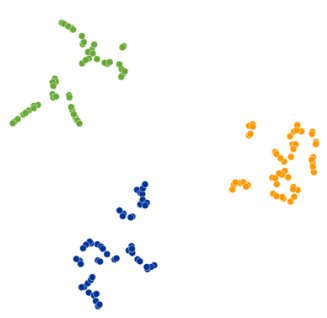
\includegraphics[scale=0.3]{abb/t-sne-example.png}
  \caption{Cluster Analyse angewendet auf 2-dimensionale Daten aus 
  \cite{wattenberg2016how}.}
\end{figure}

\subsubsection{Reinforcement Learning}
Das Reinforcement Learning ist nicht so extrem wie das unüberwachte Lernen. 
Bei diesem Paradigma liegen dem Lernalgorithmus zwar nicht die korrekten 
Output-Werte vor, aber der Lernalgorithmus erhält für jeden vorhergesagten Wert 
eine Rückmeldung, wie erwünscht dieser Wert ist. Ein Beispiel ist ein Modell,
das mittels eines Lernalgorithmus darauf trainiert wird, ein Videospiel zu 
gewinnen. Der Lernalgorithmus bekommt ein Abbild von der Umgebung und gibt dem 
Spiel einen Input, welcher eine Aktion zufolge hat. Falls nun die Aktion dazu 
beiträgt, den Spieler in eine gute Position zu bringen oder gar das Spiel zu
gewinnen, bekommt die Aktion eine positive Bewertung, andernfalls eine
negative. 

Die Problemstellung im maschinellen Lernen ist allgemein formuliert und abstrakt.
Dies ist der Grund, warum maschinelles Lernen in vielen unterschiedlichen 
Bereichen eingesetzt werden kann. Einer der Bereiche ist die linguistische
Datenverarbeitung (engl. natural language processing), was uns zum nächsten 
Begriff führt. Linguistische Datenverarbeitung wird im Folgenden mit NLP abgekürzt.

\subsection{Semantische Vekorräume}
Das semantische Codieren von natürlicher Sprache in einem Vektorraum 
ist ein bedeutsames Problem in NLP. %Referenz?
Der resultierende Vektorraum kann
für verschiedene Problemstellungen (engl. downstream tasks) verwendet
werden. Ein Beispiel ist die Klassifizierung von Spam Nachrichten 
\cite{Ball2019}.
Semantischer Vektorraum heißt hier, dass ähnliche Wörter, also Wörter 
mit ähnlicher Bedeutung, im projizierten Vektorraum einen geringen 
Abstand zueinander haben. Wir werden die Vektoren im Folgenden als
Embeddings bezeichnen. In einem idealen semantischen Vektorraum würde 
die Beziehung gelten, die in Figur 2.4 dargestellt wird.
\begin{figure}[H]
  \begin{center}
      \begin{tikzpicture}
        \draw[thin,gray!40] (-3,-3) grid (3,3);
        \draw[->] (-3,-3)--(3,-3) node[right]{$x_1$};
        \draw[->] (-3,-3)--(-3,3) node[above]{$x_2$};
        \draw[line width=2pt,red,-stealth](-2,-2)--(1,-2) 
            node[midway, below]{weiblich};
        \draw[line width=2pt,red,-stealth](-1,1)--(2,1) 
          node[midway, above]{weiblich};
        \draw[line width=2pt,blue,-stealth](-2,-2)--(-1,1) 
            node[midway, left]{Geschichtsstudium};
        \draw[line width=2pt,blue,-stealth](1,-2)--(2,1) 
          node[midway, right]{Geschichtsstudium};
        \filldraw (-2,-2) circle (2pt)
        node[anchor=north east]{Mann};
        \filldraw (1,-2) circle (2pt)
        node[anchor=north west]{Frau};
        \filldraw (-1,1) circle (2pt)
        node[anchor=south east]{Taxifahrer};
        \filldraw (2,1) circle (2pt)
        node[anchor=south west]{Taxifahrerin};
    \end{tikzpicture}
  \end{center}
  \caption{Optimaler fiktiver semantischer Vektorraum}
\end{figure}
\subsubsection{Bag-of-Words}
Der naivste Ansatz ist es, jedem Wort im vorliegenden Text eine Zahl 
zuzuordnen. Dadurch können sowohl die Häufigkeit eines Wortes als auch
die Sätze, in denen ein bestimmtes Wort vorkommt, effizient gefunden 
werden. Die Bedeutung eines Wortes ist hier komplett unabhängig von 
der Wahl der zugewiesenen Zahl. Das führt dazu, dass sogar Synonyme einen
hohen Abstand haben können.

\begin{example}
  Sei $T = \{\text{Input}, \text{Mann}, \text{Frau},
   \text{Eingabe}\}$ eine Menge von Wörtern, dann ist die Zuordnung
  zu dem Vektorraum $\mathbb{N}^1$ wie folgt:
  \[
    \text{Input} \to 1, 
    \text{Mann} \to 2, 
    \text{Frau} \to 3,
    \text{Eingabe} \to 4.
  \]
  Obwohl Eingabe und Input semantisch sehr ähnlich sind, haben sie hier
  einen sehr unterschiedlichen Wert.
\end{example}
\subsubsection{Word2Vec}
Im Jahr 2013 veröffentlichten Mikolov et al.  
\cite{word2vec},
zwei Modellarchitekturen, mit der ein
neuronales Netzwerk effizient lernen kann, semantische Embeddings
zu produzieren.
Mirkolov et al. haben eine Implementierung veröffentlicht die sie 
\textit{Word2Vec} \footnote{https://code.google.com/archive/p/word2vec/}
genannt haben.
In beiden Architekturen besteht das neuronale Netzwerk aus einem 
Hidden Layer, der nach dem Training die reellwertigen 
Vektorrepräsentationen enthält.
Der Aufbau bei beiden Modellen ist in Figur 2.5 dargestellt.
Es ist zu beachten, dass der Hidden Layer keine Aktivierungsfunktion 
besitzt, da er nur als lineare Transformation von einer 
One-Hot-Codierung zu einem reellwertigen Vektor dient.

One-Hot-Codierung produziert für jedes aus n Wörtern einen Vektor
$v \in \{0,1\}^n$. Dieser Vektor ist an einer Stelle mit einer Eins
und sonst überall mit einer Null versehen. Jede Position, an der eine
Eins ist, gibt es nur einmal und codiert so durch die Position ein Wort.
Der Output-Layer hat als Aktivierungsfunktion einen Softmax, der 
Softmax gibt Werte zwischen 0 und 1 zurück. Der Output ist also ein 
Vektor $v \in (0,1)^n$, daraus kann dann entweder je nach Anwendung 
durch One-Hot-Codierung ein oder mehrere Wörter abgeleitet werden.

\begin{figure}[H]
  \begin{center}
    \begin{tikzpicture}
    [inner sep=2mm,
     place/.style={circle,draw=blue!50,fill=blue!20,thick},
     transition/.style={rectangle,draw=black!50,fill=black!20,thick}]
    \node (i1) at (-3,4) {$1$};
    \node (i2) at (-3,2) {$0$};
    \node (dotsi1) at (-3,1) {$\vdots$};
    \node (i3) at (-3,0) {$0$};
    \node (L11) at (-1,4) [place] {$I_1$};
    \node (L12) at (-1,2) [place] {$I_2$};
    \node (dots1) at (-1,1) {$\vdots$};
    \node (L13) at (-1,0) [place] {$I_n$};

    \node (L21) at (2,4) [place] {$H_1$};
    \node (L22) at (2,2) [place] {$H_2$};
    \node (dots2) at (2,1) {$\vdots$};
    \node (L23) at (2,0) [place] {$H_n$};

    \node (L31) at (5,4) [place] {$O_1$};
    \node (L32) at (5,2) [place] {$O_2$};
    \node (dots3) at (5,1) {$\vdots$};
    \node (L33) at (5,0) [place] {$O_n$};

    \node (o1) at (7,4) {$0.1$};
    \node (o2) at (7,2) {$0.3$};
    \node (dotso1) at (7,1) {$\vdots$};
    \node (o3) at (7,0) {$0.8$};

    \draw[->] (i1) -- (L11);
    \draw[->] (i2) -- (L12);
    \draw[->] (i3) -- (L13);

    \draw[->] (L11) -- (L21);
    \draw[->] (L11) -- (L22);
    \draw[->] (L11) -- (L23);
    \draw[->] (L12) -- (L21);
    \draw[->] (L12) -- (L22);
    \draw[->] (L12) -- (L23);

    \draw[->] (L13) -- (L21);
    \draw[->] (L13) -- (L22);
    \draw[->] (L13) -- (L23);

    \draw[->] (L21) -- (L31);
    \draw[->] (L21) -- (L32);
    \draw[->] (L21) -- (L33);

    \draw[->] (L22) -- (L31);
    \draw[->] (L22) -- (L32);
    \draw[->] (L22) -- (L33);

    \draw[->] (L23) -- (L31);
    \draw[->] (L23) -- (L32);
    \draw[->] (L23) -- (L33);

    \draw[->] (L31) -- (o1);
    \draw[->] (L32) -- (o2);
    \draw[->] (L33) -- (o3);
    \end{tikzpicture}
    \caption{ Architektur des neuronalen Netzwerks von Word2Vec}
  \end{center}
\end{figure}
Es gibt nun zwei unterschiedliche Strategien, das neuronale Netzwerk
zu trainieren. Die erste ist Skip-Gram, gegeben ein Wort, muss das
Modell die naheliegenden Wörter vorhersagen. Das heißt, es muss einem
Wort einen richtigen Kontext zuordnen. Das Modell wird die Fähigkeit
entwickeln, Wörter mit ähnlichen Kontexten ähnlichen Embeddings
zuzuordnen. 

Die zweite Methode ist Continous Bag-of-Words (CBOW),
bei der das Modell Wörter nahe an einem bestimmten Wort als Input 
erhält und versucht, dieses Wort vorherzusagen.Folglich muss das Wort,
das in dem gegebenen Kontext verwendet wird, prädiziert werden.
Da ähnliche Wörter ähnliche Kontexte haben, neigt das Modell dazu,
ähnliche Outputs für ähnliche Kontexte zu lernen. 

Die Word2Vec-Embeddings sind dann ähnlich, wenn ihre Kontexte,
in denen sie verwendet werden, ähnlich sind.  
Die Kontexte haben eine feste Größe, die am Anfang ausgewählt wird.
Wenn die Kontextgröße zu klein gewählt wird, kann es passieren, dass 
das Wort mit inhaltslosen Wörtern assoziiert wird, wie z.B. Artikel 
oder Präpositionen. Wenn die Kontextgröße zu groß ist, können 
unterschiedliche Kontexte verschwimmen und ungenaue Ergebnisse entstehen.
Folglich hat die Kontextgröße einen entscheidenden Einfluss auf den Erfolg 
des Modells. Vaswani et al. lösen das Kontextproblem 
durch die Transformer-Modellarchitektur  \cite{transformer}.

\subsubsection{Transformer}
Die Transformer-Architektur \cite{transformer}
ist ein Meilenstein im NLP Bereich.
Die vorgestellte Deep Learning Architektur bildet die Basis für BERT,
\textit{SentenceTransformer} und Large Language-Models (wie z.B. Chat-GPT).
Das Modell wurde ursprünglich entwickelt, um bei einem gegebenen Satz 
einen sinnvollen neuen Satz zu generieren. Die Donwstream Task auf die 
eine Implementierung der Architektur trainiert wurde,
ist das Übersetzen von Englisch zu Deutsch oder Französisch. 
Der Transformer kann jedoch wieder zur Erzeugung semantischer Embeddings 
verwendet werden, wie wir im Abschnitt zum \textit{SentenceTransformer} sehen 
werden.
\begin{figure}[H]
  \begin{center}
    \begin{tikzpicture}
      [inner sep=2mm,
       place/.style={circle,draw=blue!50,fill=blue!20,thick},
       transition/.style={rectangle,draw=black!50,fill=black!20,thick}]
        \node (E) at (-2,0) [transition] {Encoder};
        \node (D) at (2,0) [transition] {Decoder};
        \node (I) at (-2,-2) {Input};
        \node (O) at (2,2) {Output};
        
        \draw[->] (I) -- (E);
        \draw[->] (E) -- (D);
        \draw[->] (D) -- (O);
        \draw[->] (O) -- (D);
      \end{tikzpicture}
  \end{center}
  \caption{Transformer-Architektur stark vereinfacht}
\end{figure}
Die Architektur hat zwei große Blöcke, die in der Abbildung 2.6 zusehen
sind. Der erste Block ist der Encoder, dieser erhält die Eingabe.
Beim Übersetzen wäre das der zu übersetzende Text.
Der Encoder codiert den Input in semantische Embeddings und gibt an,
wie wichtig jedes Wort in dem Satz für ein gegebenes Wort ist.
Es gibt keine Kontextgröße, sondern der Kontext ist die gesamte
Eingabe.
Der Encoder bestimmt, welche Wörter wichtig sind und welche eher 
unwichtig sind in Bezug auf ein gegebenes Wort.
Der Decoder erhält den von ihm selbst produzierten Output sowie 
das Ergebnis des Encoders, um das nächste Wort zu generieren. 
Außerdem startet dieser mit einem konstanten Start-Embedding und 
um die Generierung zu stoppen, gibt er selbst ein konstantes 
Stopp-Embedding aus. Es ist wichtig, dass mehrere Encoder und Decoder 
gleichzeitig hintereinander geschaltet werden können.

Die Architektur ist in Abbildung 2.7 dargestellt. Im Folgenden werden 
die wichtigsten Bestandteile der Abbildung erläutert. {\bf Input-Embedding}
gibt dem Input, der in Textform vorliegt, eine Vektorrepräsentation.
Danach wird auf dem Vektor ein {\bf Positional Encoding} darauf addiert.
Der Transformer verarbeitet alle Wörter parallel, deswegen geht die 
Positionsinformation verloren. Um diese Information trotzdem im Vektor 
zu codieren, wird für jede Position ein einzigartiger Vektor darauf 
addiert. Im Block {\bf Add \& Norm} werden zwei Inputs addiert und dann 
normalisiert, damit die Werte in dem Modell nicht zu groß werden.
Feed Forward ist einfach ein neuronales Netzwerk mit zwei Layern.
Alle Wort-Embeddings werden nacheinander und identisch in das Netzwerk 
eingegeben. Der erste Input-Layer hat als Aktivierungsfunktion ein 
Softmax und der zweite hat die Identitätsfunktion.
Dann gilt für das Netzwerk:
\[
  FFN(x) =\text{max}(0, xW_1 + b_1)W_2 + b_2.
\]
Der {\bf Linear Block} ist wieder ein neuronales Netzwerk, mit allen
Aktivierungsfunktionen: $ f_{i,j}(x) = x $. 
Das {\bf Multi Head-Attention} Modul ist der wohl wichtigste Bestandteil der 
Architektur. Dieses gibt die Korrelation zwischen einem Wort und allen
Restlichen im Input aus. Der gesamte Input wird als Kontext betrachtet,
aber das Modell lernt, auf welche Wörter es im Kontext viel oder wenig
Aufmerksamkeit schenken sollte. Das {\bf Masked Multi Head-Attention}
Modul ist nur beim Trainieren anders als das Multi Head-Attention-Modul.
Beim Trainieren ist der Input des Decoders bereits der Satz,
den das Modell vorhersagen soll. Daher müssen alle Wörter, 
die es noch nicht vorhergesagt hat, verdeckt (engl. masked) werden.
\begin{figure}[H]
  \begin{center}
    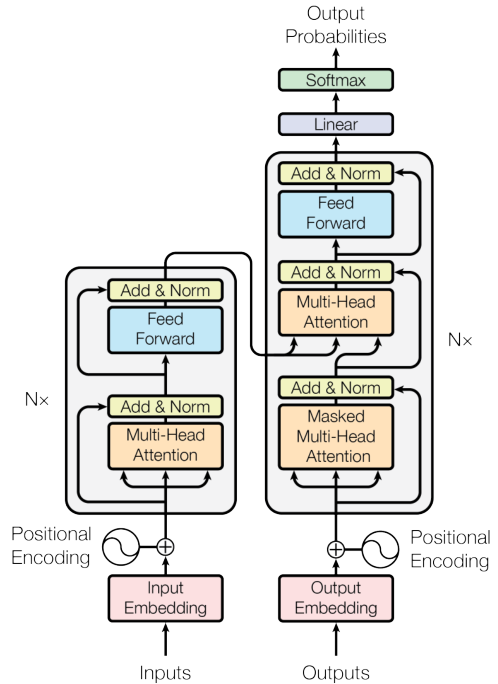
\includegraphics[scale=0.35]{abb/transformer-figure.png}
  \end{center}
  \caption{
      Transformer-Architektur entnommen aus \cite{transformer}.
      Der linke Block ist der Encoder und der rechte Block der Decoder.
  }
\end{figure} 
\subsubsection{BERT}
Das BERT-Modell \cite{conf/naacl/DevlinCLT19} 
ist ein wichtiger Meilenstein im NLP-Bereich und kann 
als eines der ersten Large Language-Models betrachtet werden.
Das Modell verbessert die Transformer-Architektur, 
indem es die Token-Embeddings verbessert, zwei neue Trainingsaufgaben einführt
und ausschließlich Encoder verwendet.
\begin{figure}[H]
  \begin{center}
    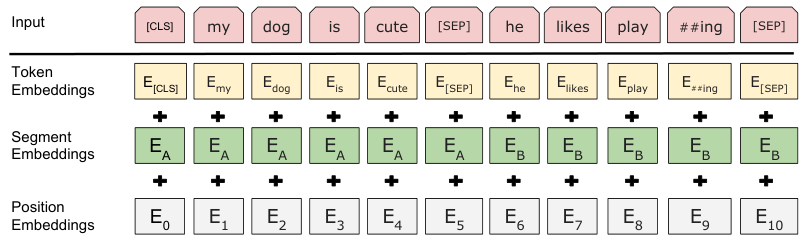
\includegraphics[scale=0.5]{abb/BERT-Tokens.png}
  \end{center}
  \caption{
    Token-Embedding-Prozess entnommen aus 
    \cite{conf/naacl/DevlinCLT19}.
  }
\end{figure}
In Abbildung 2.8 ist der Token-Embedding-Prozess abgebildet,
der im Folgenden näher beschrieben wird. Zunächst muss erläutert werden, 
was ein Token ist. Ein Token ist in diesem Fall ein Wort, 
aber generell ist ein Token eine kleinere Zeichenkette, die aus einem 
Text gewonnen wird und einer Bedeutung zugewiesen wird oder in eine 
Zahl umgewandelt wird, um die Weiterverarbeitung zu vereinfachen.

Das BERT Modell kombiniert drei unterschiedliche Informationen
in Vektorform, um noch bessere Token-Embeddings zu generieren. BERT
verwendet \textit{WordPiece} \cite{wu2016googlesneuralmachinetranslation},
um die Token-Embeddings zu erhalten.
Auf diese werden nun ein Segment-Embedding und schließlich die
Position-Embeddings addiert. {\bf Segment-Embedding} codiert die Information,
welche Tokens strukturell zusammen gehören (Bspw. ein Satz).
Das {\bf Position-Embedding} codiert die sequenzielle Position im Input.


Die beiden unterschiedlichen Trainingsaufgaben stellen das wichtigste
Puzzleteil dar. Während der Transformer die Tokens von links nach rechts
vorhersagt, wird BERT darauf trainiert, Wörter vorherzusagen, die auf
beliebiger Position fehlen. Dadurch erhält das Modell Zugang zu dem
Kontext, der sich links und rechts von dem zu prädizierenden Token befindet.
Wu et al. benennen diese Trainingsform {\bf Masked Language-Modeling}.
Bei diesem Verfahren werden $15 \%$ der Input-Token entweder durch das
\verb|[Mask]| Token oder durch einen zufälligen anderen Token ersetzt.
Dabei werden $10 \%$ der Token, die maskiert werden sollten,
unverändert bleiben. Weitere $10 \%$ werden durch ein zufälliges anderes
Token ersetzt, während die restlichen $80 \%$ durch das \verb|[Mask]| Token 
ersetzt werden.
\pagebreak

Die zweite Trainingsaufgabe ist {\bf Next Sentence-Prediction} (NSP),
bei dieser Aufgabe muss das BERT Modell bei der Eingabe von zwei Sätzen 
entscheiden, ob diese sequenziell nacheinander kommen oder nicht.
Bei der einen Hälfte der Daten handelt es sich um zwei Sätze, die nacheinander 
auftreten. Bei der anderen Hälfte der Daten handelt es sich um zufällige,
nicht sequenzielle Sätze. Zur Vorhersage, ob die Sätze nacheinander kommen 
oder nicht, wird das konstante \verb|[cls]| Token-Embedding verwendet, 
welches beim Input immer an erster Stelle steht. Der erste Output-Vektor 
ist dann das Ergebnis des \verb|[cls]| Tokens und wird verwendet, um den Output
\verb|isNext| oder \verb|notNext| zu produzieren.

Nach dem Training erhält man aus BERT für jeden Input-Vektor genau einen 
Output-Vektor, diesen kann man dann mit wenig Aufwand weiter verwenden,
um das Modell für bestimmte Probleme in NLP anzupassen 
(engl. fine tuning).

\subsubsection{Sentence Transformer}
Das Sentence-BERT \cite{reimers-2019-sentence-bert}
Modell ist der aktuelle Stand der Technik im semantischen Codieren von 
natürlicher Sprache in einem Vektorraum. Die Implementierung von 
Reimers et al.
ist unter dem Namen \textit{SentenceTransformer} 
\footnote{https://sbert.net}
bekannt. Die Motivation 
hinter Sentence-BERT (SBERT) ist das effiziente semantische Vergleichen 
von zwei Sätzen. Wenn man mit BERT herausfinden möchte, wie semantisch
ähnlich zwei gegebene Sätze sind, dann muss man beide Sätze als Input 
in das Modell eingeben. Das heißt, wenn man die Ähnlichkeit von allen
$n$ Sätzen jeweils zueinander haben will, gibt es $\frac{n(n-1)}{2}$ 
Eingaben in das BERT Modell, die man tätigen müsste.
Bei SBERT kann dagegen jeder Satz einzeln eingegeben werden und der
resultierende Output ist dann ein semantischer Vektorraum, indem jeder 
Satz einen semantischen Vektor besitzt. Um die semantische Ähnlichkeit 
zwischen zwei Vektoren zu erhalten, müssen beide Vektoren lediglich in 
eine zu wählende Metrik eingesetzt werden. 
%wird die Kosinus-Ähnilichkeit verwendet: Sei $u,v \in \mathbb{R}^n$, dann setze
%\[
%  Kos(u,v) := cos(\phi) = \frac{u \cdot v}{\|u\|\|v\|} 
%  = \frac
%  {
%    \sum_{i=1}^n u_iv_i
%  }
%  {
%    \sqrt{\sum_{i=1}^n u_i^2} \sqrt{\sum_{i=1}^n v_i^2}
%  }.
%\]
Dies ermöglicht es, die semantische Ähnlichkeit zwischen zwei Vektoren 
effizient zu berechnen.

Die Modellarchitektur von SBERT wird als {\bf Siamese Neural Network }
bezeichnet, da zwei unterschiedliche BERT-Modelle verwendet werden,
um beide Sätze in einen Vektor umzuwandeln, aber beide Modelle teilen 
sich die Gewichte.
\pagebreak

\begin{figure}[H]
  \begin{center}
    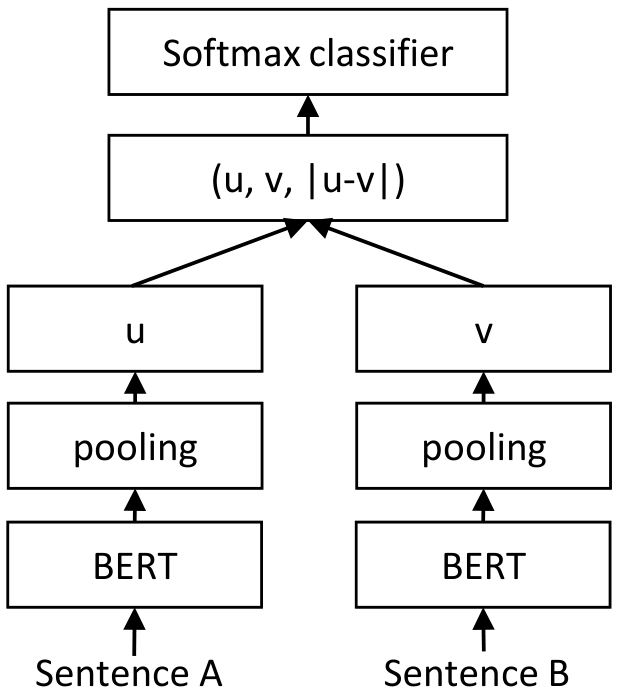
\includegraphics[scale=0.3]{abb/SBERT.png}
  \end{center}
  \caption{
    SBERT-Architektur entnommen aus \cite{reimers-2019-sentence-bert}. 
    Beide BERT-Modelle teilen sich dieselben Gewichte. 
  }
\end{figure}
Danach geht der Output von BERT in ein Pooling-Modul. 
{\bf Pooling} ist das Transformieren von Output mit vielen Vektoren 
in eine geringere Anzahl von Vektoren oder Dimensionen. In diesem Fall 
werden die $n$ Output-Vektoren von BERT in einen einzigen Output-Vektor 
transformiert. Das Default Pooling ist der Mittelwert, d.h. auf alle 
Output-Vektoren von BERT wird das arithmetische Mittel angewendet.
Daraus erhält man einen Vektor mit den jeweiligen gemittelten 
BERT-Output-Vektoren.

Das BERT Modell wird an die spezielle Aufgabe 
angepasst, zwei Vektoren semantisch zu vergleichen. 
Dafür wird der SNLI Datensatz verwendet, dieser beinhaltet immer 
zwei Sätze und eins von drei möglichen Labels: 
\verb|contradiction|, \verb|neutral|, und \verb|entailment|.
SBERT muss für zwei Sätze vorhersagen, ob sie sich inhaltlich widersprechen,
neutral zueinander sind oder ob der eine Satz eine Fortsetzung des 
anderen ist. Daraus lernt das Modell, ein semantisches Verständnis 
für Sätze zu erlangen. Zur Ermittlung der Label-Vorhersage werden die 
jeweiligen Vektoren und ihre Differenz konkateniert. Anschließend 
werden diese mit einem, durch Training erlernten, Gewicht multipliziert,
sodass ein 
Vektor mit drei Dimensionen entsteht. Danach wird der Softmax auf das
Ergebnis angewendet. Die Position in dem Vektor mit dem höchsten Wert 
wird schließlich dem zugehörigen Label zugeordnet. Mathematisch:
Sei $W \in \mathbb{R}^{n\times 3}$ das Gewicht und 
$v \in \mathbb{R}^n$ Output-Vektor von dem Pooling, dann
\[
  o = \text{softmax}(Wv).
\]
Nachdem Training bei der Inferenz wird der Vektor, nachdem Pooling 
als Output-Vektor ausgeben. SBERT liefert uns also ein Tool, 
um Sätze semantisch in einem Vektorraum abzubilden,
welches sich in späteren Kapiteln als sehr hilfreich herausstellt.
\pagebreak
\subsection{Code Llama}
Die \textit{Code Llama} Familie an Large Language-Models wurde von 
Rozière et al. bei Meta AI im Jahre 2024 entwickelt
\cite{rozière2024codellamaopenfoundation}.
{\bf Large Language-Models} sind Modelle, die auf
einer großen Menge von Daten trainiert wurden, welche sich darin
auszeichnen, natürliche Sprache verstehen sowie generieren zu
können und deswegen in der Lage sind, eine Vielzahl von Aufgabe
n im NLP-Bereich zu lösen.

Meta AI optimiert das vorangegangene Llama-2-Modell auf
Programmiersprachen spezifische Aufgaben. Das LLama-2-Model wird,
um zum resultierenden Code Llama zu kommen, erneut auf einem neuen
Datensatz trainiert. Dieser besteht aus drei verschiedenen 
Kategorien von Daten. Der größte Teil im Datensatz, mit $85 \%$,
ist mit Programmiersprachen spezifischen Aufgaben verbunden,
indem das Modell darauf trainiert wird, fehlende Programmzeilen in 
einer vergebenen Lücke zu füllen. Dabei kann es sich um Programmcode,
aber auch um Kommentare handeln. Der zweitgrößte Teil im Datensatz,
mit $8 \%$, besteht aus natürlicher Sprache, in der es um 
Programmcode geht. Dieser Teil beinhaltet Diskussion über Quellcode
sowie Fragen und Antworten, welche sich auf Quellcode beziehen. 
Der kleinste Teil im Datensatz mit $7 \%$ besteht aus beliebiger 
natürlicher Sprache, damit das Modell seine alten Fähigkeiten erhält. 

Das LLama-2-Modell ist eine Verbesserung des Llama-Modells.
Dieses wurde auf neueren Daten trainiert und verwendet einen 
$40 \%$ größeren Datensatz. Zudem wurde die maximale Anzahl 
der gleichzeitig zu verarbeitenden Token verdoppelt. Außerdem 
gab es eine Veränderung in der Llama-Transformer-Architektur. 
In den Attention-Modulen werden zwei Werte, die normalerweise 
immer wieder berechnet werden, geteilt, was bedeutet, dass 
jedes Attention-Modul Zugriff auf die gleichen Werte hat.
Dies führt zu geringfügig schlechteren Ergebnissen, jedoch zu
einer deutlichen Leistungssteigerung.

Das Llama-Modell wiederum besteht aus einer Decoder-only-Transformer-Architektur.
Der {\bf Decoder-only-Transformer}
besteht lediglich aus Decoder-Transformer-Blöcken,
wie der Name bereits vermuten lässt. Bei dieser Architektur
ist der anfängliche Input des Decoders die Eingabe des Nutzers.
Auf diese Eingabe wird dann immer wieder das neu generierte Token
drauf konkateniert. Auf diese Weise wird die Eingabe nicht explizit
von dem bereits generierten getrennt, sondern beides wird als 
gleicher Kontext verwendet.

Das Besondere an Llama ist, dass es nur auf frei verfügbaren
Daten trainiert wurde und dass das Modell Open Source ist. Der
Datensatz besteht aus English Common Crawl [$67\%$],
f C4 [$15\%$],  Github [$4.5\%$],
Wikipedia [$4.5\%$], Gutenberg and Books3 [$4.5\%$], 
ArXiv [$2.5\%$], und Stack Exchange [$2\%$].

Code Llama ist eine Open Source-Software, die unter allen 
verfügbaren Modellen am besten in multilingualen Benchmarks 
abschneidet. Multilingual bedeutet die Verwendung mehrerer 
Programmiersprachen. Diese Eigenschaften machen es sehr geeignet
für diese Arbeit.
\subsection{Code2Vec}
 \textit{Code2Vec}  ist eine im Jahre 2018 von Alon et al. 
entwickelte Modellarchitektur, die Quellcode in einen semantischen 
Vektor kodiert
\cite{code2vec}.
Nach den Erfolgen in NLP, natürliche Sprache 
in semantische Vektoren zu kodieren, entstand der Wunsch, auch 
Quellcode in semantischen Vektoren abzubilden. Mit diesen Vektoren 
können dann wieder viele verschiedene Aufgaben gelöst werden.
Das motivierende Beispiel bei \textit{Code2Vec} ist die Vorhersage 
eines sinnvollen Namens für eine Funktion. Die Architektur, welche 
in Abbildung 2.10 dargestellt ist, wird im Folgenden erläutert. 
\begin{figure}[H]
  \begin{center}
    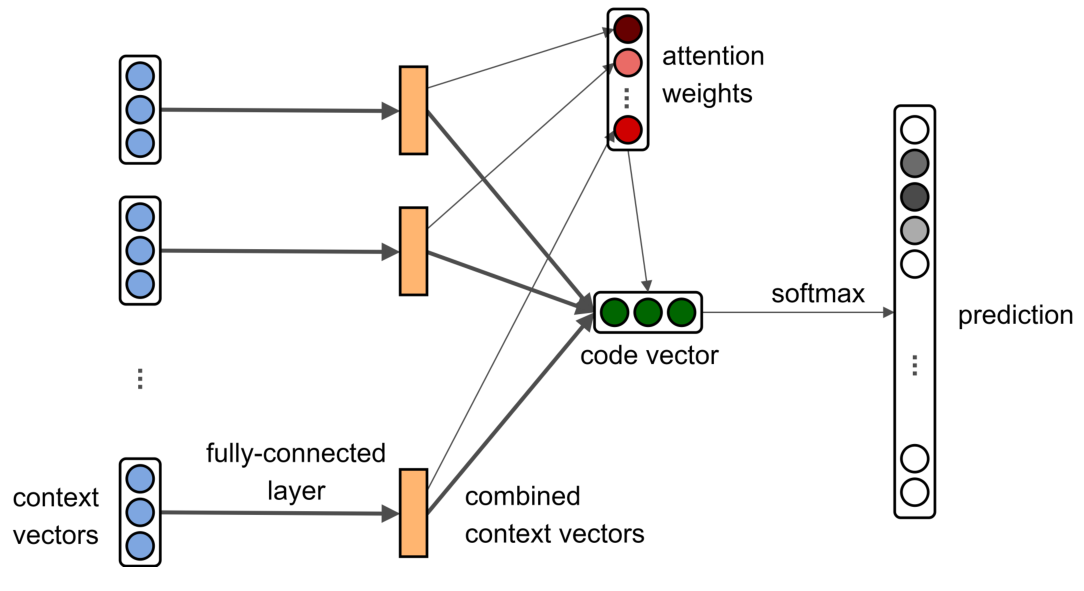
\includegraphics[scale=0.3]{abb/code2vec.png}
  \end{center}
  \caption{
    \textit{Code2Vec}-Architektur entnommen aus
    \cite{code2vec}
  }
\end{figure}
Alon et al. fanden heraus, dass eine geeignete Darstellung
von Quellcode als ein mathematisches Objekt ein abstrakter 
Syntaxbaum ist. Dieser erhält die strukturellen Zusammenhänge
zwischen den Tokens und kann gut in einen Vektor kodiert werden.
Die Input-Vektoren (Context-Vectors) bestehen jeweils aus einem
Pfad im abstrakten Syntaxbaum, mit dem jeweiligen Starttoken und
Endtoken des Pfades. Danach folgt ein Hidden Layer, mit \verb|tanh|
als Aktivierungsfunktion. Der endgültige Vektor wird als lineare 
Kombination aus den Output-Vektoren und den Attention-Weights 
berechnet. Sei $h_1, \dots, h_n \in \mathbb{R}^d$ die Output-Vektoren 
von dem Hidden Layer
und $\alpha \in \mathbb{R}^n$ der Attention-Weights Vektor.
\[
  \verb| code vector | v = \sum_{i = 1}^n \alpha_i \cdot h_i
\]

Mit dem \verb|Code-Vector| kann dann das gewünschte Label vorhergesagt 
werden. Das Modell kann demnach darauf trainiert werden, bei gegebenem 
\verb|Code-Vector| bzw. Quellcodeauszug ein bestimmtes Label in 
natürlicher Sprache vorherzusagen. Nachdem das Training abgeschlossen 
ist, kann es ein Label für einen Quellcode vorhersagen, welches nicht 
im Trainingssatz enthalten ist. 
Die Trainingsart ist demnach überwachtes Lernen, was eine Aufbereitung der
Daten benötigt. Das Modell kann lediglich die Labels vorhersagen, die es 
vorher im Training gesehen hat.

\pagebreak

\subsection{ T-Distributed Stochastic Nieigbor Embedding}
{\bf T}-Distributed {\bf S}tochastic {\bf N}eigbor {\bf E}mbedding
({\bf  t-SNE}) ist ein Algorithmus, welcher zum Visualisieren von
hochdimensionalen Daten eingesetzt wird
\cite{JMLR:v9:vandermaaten08a}. Um das zu ermöglichen,
reduziert  \textit{t-SNE} die Dimension von $n \in \mathbb{N}$ zu einer niedrigeren 
Dimension wie zwei oder drei, in der der Mensch die Datenpunkte leicht 
interpretieren kann. Dabei versucht der Algorithmus, die
Nachbarschaftsverhältnisse der Datenpunkte nicht in Mitleidenschaft zu 
ziehen.

Im Folgenden wird der Algorithmus skizziert und danach wird aufgezeigt,
was bei der effektiven Verwendung von  \textit{t-SNE} zu beachten ist. Die
hochdimensionalen Datenpunkte werden mit $\mathbf{H}$ und die niedrig 
dimensionalen Datenpunkte mit $\mathbf{N}$ bezeichnet. Der erste Schritt 
des Algorithmus ist es, jedem Datenpunktpaar im Datensatz $\mathbf{H}$
einen Ähnlichkeitsscore zuzuweisen. Dieser wird berechnet, indem man 
zuerst die euklidische Distanz von jedem Datenpaar berechnet und dann das 
Ergebnis in eine Wahrscheinlichkeitsverteilung eingibt. Dies führt zu
einer Normalisierung des Wertes. Das Ergebnis ist dann eine Tabelle mit 
einem Ähnlichkeitsscore für jedes Datenpaar in $\mathbf{H}$. 

Als Nächstes werden die Datenpunkte zufällig in der niedrigen Dimension $\mathbf{N}$
angeordnet. Die nachfolgenden zwei Schritte werden $T\in \mathbb{N}$ 
mal wiederholt, wobei $T$ ein Parameter ist, der wählbar ist.
\begin{enumerate}
  \item Berechne Ähnlichkeitsscore von $\mathbf{N}$, diesmal wird aber die
      studentische t-Verteilung als wahrscheinlichkeitsverteilung genommen. 
  \item Verschiebe die Datenpunkte von $\mathbf{N}$ um ein kleinen Wert in
    die Richtung, die den Unterschied der Ähnlichkeitsscores von $\mathbf{H}$
    und $\mathbf{N}$ minimiert.
\end{enumerate}
Nach $T$ Wiederholung ist der Ähnlichkeitsscore von $\mathbf{N}$ und 
$\mathbf{H}$ nahe bei einander, d.h. die Nachbarschaftsverhältnisse 
von $\mathbf{N}$ und $\mathbf{H}$ sind nun ähnlich.

Wattenberg et al. haben untersucht, wie man  \textit{t-SNE} sinnvoll
anwendet und welche Schlüsse man aus der Visualisierung 
ziehen kann \cite{wattenberg2016how}. 
Sie fanden heraus, dass die Wahl der Parameter 
für das Ergebnis eine wichtige Rolle spielt. Die wichtigsten 
Parameter sind die Iterationen $T\in \mathbb{N}$ und die Perplexity 
$P \in \mathbb{N}$. 

Eine geeignete Iteration $T$ kann relative einfach durch ausprobieren 
herausgefunden werden: Falls sich die Datenwolke bei Erhöhung
von $T$ nicht mehr wirklich verändert, ist die Anzahl der Iteration
$T$ gefunden. 
\pagebreak

Die Perplexity kann intuitiv als Schätzung für die Anzahl an nahen 
Nachbarn, die jeder Datenpunkt hat, gesehen werden.
Die Suche nach einer geeigneten Perplexity ist schwieriger, 
da wir die hochdimensionalen Nachbarschaftsbeziehungen häufig 
nicht kennen. Van der Maaten et al., welche  \textit{t-SNE} entwickelt haben,
empfehlen eine Perplexity $P \in \{5,6, \dots, 50\}$ 
\cite{JMLR:v9:vandermaaten08a}.
Außerhalb dieses Bereichs kann es zu unerwünschten Ereignissen 
kommen. Bei $P=2$ haben Wattenberg et al. herausgefunden, 
dass  \textit{t-SNE} bei einer zufällig generierten Datenwolke 
fälschlicherweise kleine Gruppierungen (engl. cluster) bildet. 
Falls $P$ größer ist als die Anzahl der Datenpunkte, ist das
Ergebnis überhaupt nicht interpretierbar. Es ist daher ratsam,
mehrere Werte für $P$ zu verwenden, um sicherzustellen, 
dass  \textit{t-SNE} keine falschen Nachbarschaftsbeziehungen darstellt.

Wattenberg und Kollegen stellten außerdem fest, dass sowohl die 
Information des Durchmessers eines Clusters als auch die Abstände 
zwischen einem Cluster und einem anderen durch  \textit{t-SNE} vollständig 
verloren gehen. Nach Betrachtung der  \textit{t-SNE} Ausgabe kann daher 
keine Aussage über den Durchmesser eines Clusters, die Position 
des Clusters und die Lagebeziehungen zwischen Clustern getroffen 
werden. 

Der  \textit{t-SNE} Algorithmus ist ein wichtiges Tool, um qualitative 
Aussagen über Daten zu treffen. Es ist jedoch wichtig, mehrere 
Parameter auszuprobieren. Es kann nur eine Aussage über die 
Existenz von Clustern gemacht werden, nicht über ihre geometrischen 
Gegebenheiten. Wenn diese Bedingungen beachtet werden, kann  \textit{t-SNE}
ein mächtiges Visualisierungs-Tool sein, um eine Intuition für die
Anordnung der Datenpunkte zu erlangen.

% effective use paper: 
% https://distill.pub/2016/misread-tsne/?_ga=2.135835192.888864733.1531353600-1779571267.1531353600
%pgf plots

%\subsection{Stand der Technik} in Introduction
% Self supervised learning (JTrans, PalmTree)
% Same Source policy (Safe)
%  Clap
\section{Methodik}
\subsection{Datensatz}
Im maschinellen Lernen hat der Datensatz bzw. die Trainingsdaten
den größten Einfluss auf die Güte des Modells. Wir haben uns 
für die Open Source-Standard-C-Bibliothek von GNU entschieden. 
Die Sprache C wurde gewählt, da sie die zweitpopulärste Sprache 
nach C++ ist, die zu Maschinencode kompilierbar ist.
Die GNU-Bibliothek wurde aufgrund der hohen Qualität des 
Quellcodes ausgewählt, da das Projekt seit 1987 existiert 
und die Community jederzeit auf Fehler im Quellcode hinweisen kann.
Zum anderen wird die Bibliothek weitgehend in vielen Applikationen 
eingesetzt.

Der wichtigste Aspekt ist, dass man mit diesem Datensatz 
die Ergebnisse des trainierten Modells vergleichen kann, da die 
C-Bibliothek im POSIX Standard festgelegt ist und mehrfach 
implementiert wurde. Dadurch erhält man mehrere hochqualitative 
Quellcodeprojekte, die die gleiche Semantik aufweisen. Die 
unterschiedlichen Implementierungen werden zu unterschiedlichem 
Assemblercode kompiliert. Deswegen kann mit unterschiedlichen 
Standard-C-Bibliotheken, die den POSIX Standard implementieren,
getestet werden, ob das finale Modell beide Implementierungen 
als sehr ähnlich klassifiziert.

% Warum ist die Auswahl des Datensatzes wichtig
% Warum Glibc? 
% Gleicher Standard mit gleicher Semantik unterschiedlich Implementierung

\pagebreak

\subsection{Datenpipeline}
Der große praktische Teil der Arbeit bestand darin, eine große 
Menge an Daten in unterschiedliche Darstellungen umzuwandeln. 
Jeder Zwischenschritt wurde gespeichert, um nicht jede Darstellung 
erneut generieren zu müssen. Im Folgenden wird die generelle Architektur,
wie Daten verarbeitet werden (engl. pipeline), vorgestellt, um einen 
Überblick über den praktischen Teil dieser Arbeit zu geben.
\begin{figure}[H]
  \begin{center}
    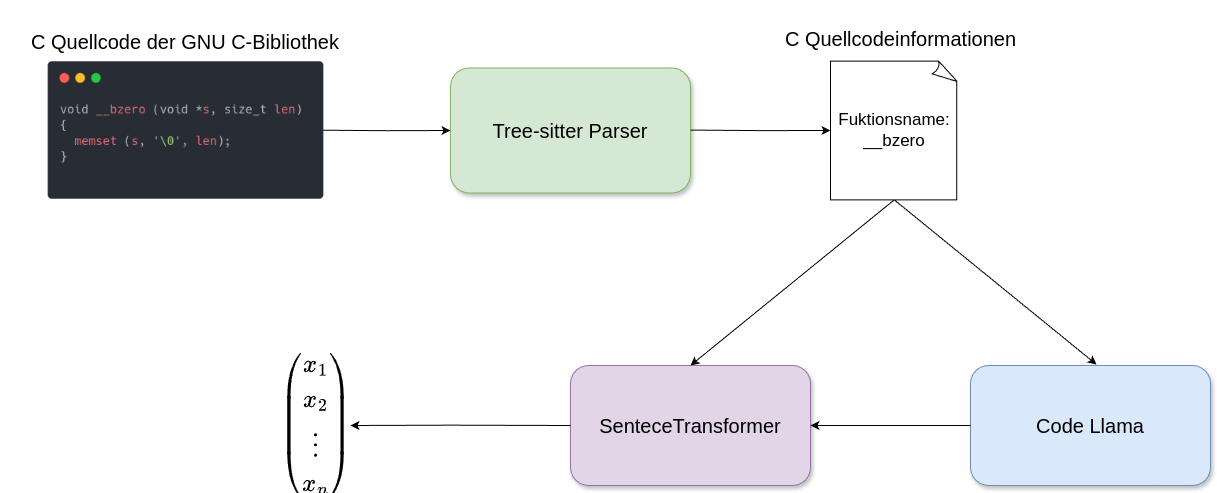
\includegraphics[scale=0.35]{abb/data-pipeline-2.drawio.png}
  \end{center}
  \caption{
    Die Datenpipeline dargestellt, dabei 
    sind Vierecke mit abgerundeten Ecken Tools, die Daten in eine 
    andere Darstellung umwandeln.
  }
\end{figure}

Die Rohdaten entsprechen dem unverarbeiteten 
C-Quellcode aus der GNU-Standard-C-Bibliothek. 
Wir benötigen nicht alle Teile des Quellcodes, sondern nur bestimmte.
Wir betrachten ausschließlich nur Funktionen, d.h. wir wollen
bspw. alle Datenstrukturen, die in dem Quellcode definiert werden,
aus dem Quellcode entfernen. Die Zerlegung und Umwandlung des
Inputs in sinnvolle Teile wird Parsing genannt.

In dieser Arbeit wurde {\bf Tree-sitter} 
\footnote{https://tree-sitter.github.io/tree-sitter/} als 
Parser verwendet, welcher
alle populären Programmiersprachen in Syntaxbäume umwandeln kann.
Ursprünglich wurde \textit{Tree-sitter} für den Texteditor Atom
entwickelt und wird heute noch in vielen Texteditoren bspw. 
für die Hervorhebung von Syntax verwendet. Generell kann 
\textit{Tree-sitter} jedoch
für alle Anwendungen benutzt werden, die Informationen aus Quellcode
verarbeiten wollen. Aus dem von \textit{Tree-sitter} generierten
Syntaxbaum kann dann jegliche gewünschte Information entnommen 
werden.

Die Quellinformationen werden immer zunächst gespeichert, damit die 
Verarbeitung beim nächsten Mal an diesem Punkt beginnen kann.
Die Quellinformationen beziehen sich immer auf eine Funktion,
deswegen bestehen die Daten aus einem Tupel, der aus je einer
Funktion und den gewünschten Quellinformationen besteht. 

Danach gibt es eine Abzweigung in der Datenpipeline, entweder 
werden die Quellinformationen von Code Llama nochmal in natürlicher 
Sprache beschrieben und dann in den \textit{SentenceTransformer}
eingegeben oder die Quellinformation wird direkt in den 
\textit{SentenceTransformer} eingegeben. Schließlich erhält man wieder 
eine Datenmenge, die aus Tupeln besteht. Ein Tupel besteht aus dem 
Funktionsnamen und dem zugewiesenen semantischen Embedding. 
Bei dieser Architektur kann mühelos jedes Tool ausgewechselt werden,
solange die Ausgabeformate eingehalten werden. 
% Treesitter erklären
% Source Code information in json datei speichern
% Dann Source code information in Vektor umwandeln
% Modularität -> Vorteile dieses Designs 
\subsection{Stabilität von SentenceTransformer}
Im vorherigen Abschnitt haben wir festgestellt, dass der endgültige
Schritt für alle Daten der \textit{SentenceTransformer} ist, deshalb
bildet 
er das Herzstück der Datenpipeline. In dieser Arbeit sollen 
verschiedene semantische Beschreibungen des Quellcodes in 
natürlicher Sprache verglichen werden. Es ist wichtig, dass alle 
anderen Elemente in der Datenpipeline konstante Ergebnisse 
liefern und nicht schwanken. Aus diesem Grund wird im Folgenden 
untersucht, wie sich der \textit{SentenceTransformer} bei selber
Eingaben verhält. Im Optimalfall sollte der SentenceTransfomer bei 
selbem Input dasselbe Ergebnis liefern.

Um dies zu überprüfen, wurden $n = 100$ Code Llama 
Quellcode-Erklärungen zufällig ausgewählt und anschließend in
den SentenceTransformer $m = 100$ Mal eingegeben. Dabei beträgt
der höchste Abstand von zwei Vektoren,
die aus der gleichen Erklärung resultiert sind 
$d = 6.661338\cdot 10^{-16}$. Der 
Abstand ist ausreichend klein, um ihn in der Evaluation zu 
vernachlässigen. Der \textit{SentenceTransformer} ist daher
für die Anwendung in dieser Arbeit ausreichend stabil.

% Label Prozess sollte stabil sein bzw. deterministisch, sonst
% kann keine aussage über die Güte der Labels getätig werden
% Tabelle mit Ergebnissen der standardabweichungen
%
\pagebreak
\subsection{Funktionskommentare}
Bevor ein Programm kompiliert wurde, gibt es eine Menge an
Informationen, die die Semantik der Funktion in natürlicher Sprache 
beschreiben. Eine offensichtliche Quellcodeinformation, die im
Optimalfall die Semantik der Funktion in natürlicher Sprache 
beschreibt, ist der Kommentar. Ein gelungener Kommentar zu einer
Funktion beschreibt die Kernfunktion der Prozedur, d.h. den Input,
den Output und die Umwandlung. Dieser Kommentar kann man dann in den 
SentenceTransformer  eingeben und  so in einen semantischen 
Vektorraum abbilden.
% Warum könnten funktionskommentare dafür geignet sein die Semantik einer
% Funktion zu beschreiben
Das Parsen der Kommentare wurden mit \textit{Tree-sitter} realisiert,
wie im Abschnitt zur Datenpipeline erwähnt. Dabei gab es eine große
Designentscheidung zu treffen, welche Kommentare in einer Funktion
berücksichtigt werden sollen.
Im Rahmen dieser Arbeit werden ausschließlich Kommentare verwendet,
die direkt  über der Funktion in stehen. Da die einzeiligen Kommentare
innerhalb der Funktion meistens keinen großen semantischen Wert haben,
sondern auf Gefahren oder Designentscheidungen  hinweisen.
%(Beleg maybe: A survey on Reasearh of code comment). 
Hierbei muss man aufpassen, dass der Prozess des Parsen nicht zu
speziell an die vorliegenden Datensatz angepasst wird, sonst 
verliert er seine Allgemeingültigkeit. 

\pagebreak
% Probleme beim Parsen, wo sucht man nach Kommentaren?
% Keine einheitliche Konvention
% -> Unterschiedliche Code Base Unterschiedliche Kommentar Konventionen
\subsection{Code2Vec}
Das Besondere an \textit{Code2Vec} ist, dass der Quellcode in einem
abstrakten Syntaxbaum kodiert wird. Dies ermöglicht die Verwendung aller
Quellcodeinformationen, die im Quellcode enthalten sind. Anschließend wird
das Modell darauf trainiert, eine Eigenschaft in natürlicher Sprache
über den Quellcode vorherzusagen.

Bei dieser Herangehensweise, semantische Vektoren zu erzeugen, wird
also kein \textit{SentenceTransformer}
verwendet, sondern die Vektorraum werden durch Training des
\textit{Code2Vec} Modells als Nebenprodukt erzeugt. Wie in dem 
\cite{code2vec} wird
das Modell auch hier darauf trainiert, Funktionsnamen 
vorherzusagen. Die Implementierung des \textit{Code2Vec} Modells
nutzte Java als Datensatz, weshalb einige Anpassungen notwendig waren,
um das Modell auf C-Code zu trainieren.

Da das \textit{Code2Vec} Modell auf überwachtem Lernen basiert,
muss der Datensatz vor dem Training zunächst aus dem rohen Quellcode 
aufbereitet werden.
% Warum könnte \textit{Code2Vec} semantisch gute Vektoren produzieren
\subsubsection{Adaption auf C}
Um das \textit{Cod2Vec} Modell zu trainieren, ist es notwendig,
aus dem rohen Quellcode einer Funktion jeweils einen abstrakten 
Syntaxbaum und den
Funktionsnamen zu extrahieren. Alon et al. stellen ein Tool 
für Java zur Verfügung, welches das Extrahieren von abstrakten 
Syntaxbäumen und Funktionsnamen aus Java-Quellcode ermöglicht.

Mit dem ASTminer von Kovalenko et al. können abstrakte Syntaxbäume und 
Funktionsnamen extrahiert werden \cite{kovalenko2019pathminer}. 
Das Tool wurde vom JetBrains-Research-Team entwickelt, um Quellcode
in abstrakte Syntaxbäume (AST) zu 
kodieren, die als Input-Format für maschinelles Lernen dienen.

Die Implementierung des \textit{Code2Vec}-Modells braucht ein bestimmtes
Format, den der Datensatz aufweisen muss. Ein Trainingsbeispiel besteht
jeweils aus einem 
Funktionsnamen, dem Label und einer Liste von Kontexten, welche den AST 
repräsentieren. Ein Kontext besteht aus einem Starttoken, einem Endtoken 
und einer Pfadbeschreibung vom Starttoken bis zum Endtoken. 


Dieses \textit{Code2Vec}-Format kann durch eine zusätzliche Option in der
Konfiguration des \textit{ASTminers} generiert werden. Obwohl diese Option 
mit "code2vec" betitelt ist, ist der Output des \textit{ASTminers} nicht direkt 
von \textit{Code2Vec} verwendbar. Das Tool weist nämlich jedem Token eine
einzigartige Zahl zu und verwendet dann im Datensatz nur noch die Zahl.
Dieses Format reduziert zwar den Speicheraufwand, aber es wird von 
\textit{Code2Vec} nicht als valide Eingabe akzeptiert. Demnach mussten noch die 
Nummern wieder zu den passenden Token umgewandelt werden.
\begin{figure}[H]
  \begin{center}
    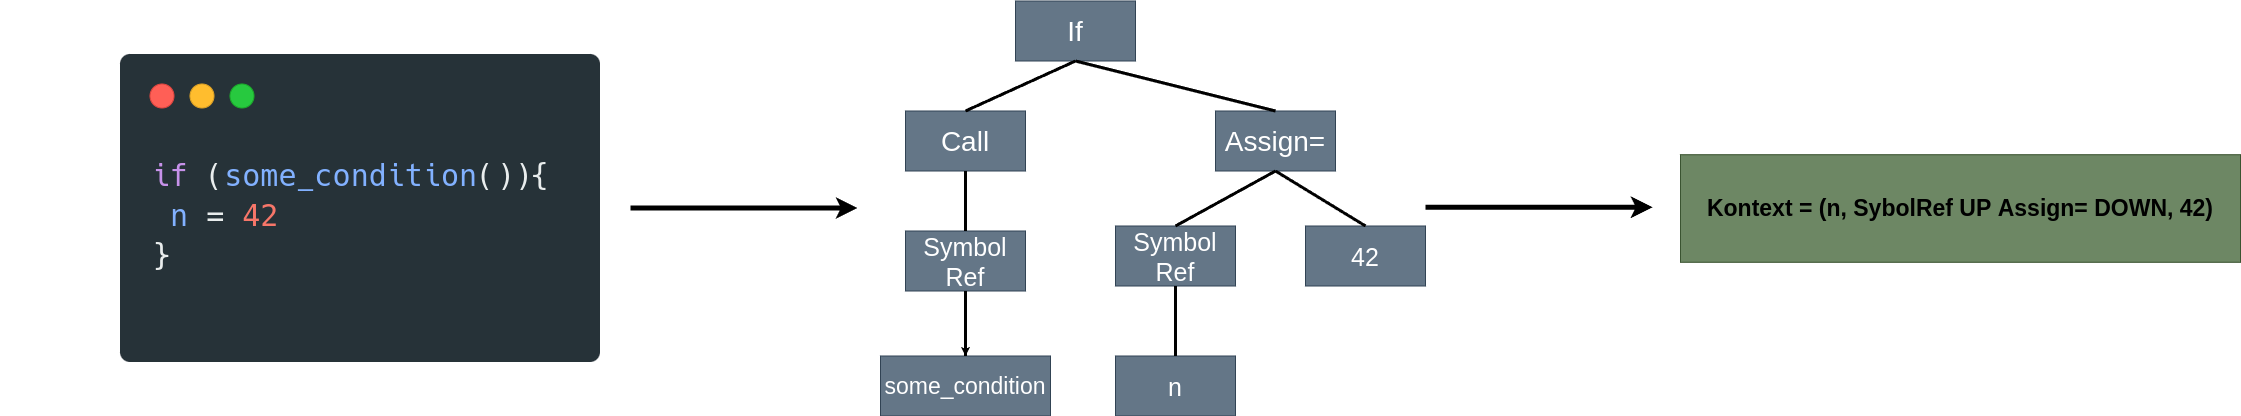
\includegraphics[scale=0.2]{abb/ast-extraction-example.drawio.png}
  \end{center}
  \caption{Extrahierung eines Kontexts aus einem C-Quellcode}
\end{figure}
Da es unterschiedliche Konventionen für Funktionsnamen gibt, wie z.B.
\verb|Camel-Case| und \verb|Snake-Case|, normalisiert der \textit{ASTminer} 
die Funktionsnamen. Dadurch sind die Trainingsdaten unabhängig von den
jeweiligen Quellcodekonventionen.
\begin{example}
  \hfill
  \begin{center}
    Snake-Case: \verb|funktions_name| $\to$ {\bf funktions\text{\textbar}name }\\
    Camel-Case: \verb|funktionsName| $\to$ {\bf funktions\text{\textbar}name}
  \end{center}
\end{example}
\textit{Code2Vec} kann nach dem Training für jede Funktion einen hochdimensionalen
Vektor ausgeben, der die Semantik der Funktion beschreiben soll.
Um mit \textit{Code2Vec} diesen Vektor generieren zu können, muss der abstrakte 
Syntaxbaum eingegeben werden. Die abstrakten Syntaxbäume können nur durch 
ihren normalisierten Namen identifiziert werden, da sie als Tupel in dieser 
Form im Datensatz vorliegen. Die normalisierten Namen können nicht mehr 
eindeutig dem initialen Funktionsnamen zugeordnet werden, da durch die 
Normalisierung Informationen verloren gehen. Zur Vergleichbarkeit von 
\textit{Cod2Vec} mit anderen Ansätzen wie z.b. Funktionskommentaren ist es notwendig,
die normalisierten Namen wieder zu den ursprünglichen Namen zurückzuführen.
Aufgrund dessen mussten im Quellcode von \textit{ASTminer} Änderungen vorgenommen 
werden, sodass zu jeder Position eines Trainingsbeispiels im Datensatz der 
ursprüngliche Funktionsname zugeordnet werden kann. 

% Code ändern bei astminer um die Namen der Funktionen am ende zuzordnen zu können
% da die Namen normalisiert werden und nicht mehr eindeutig zugeordnet werden können
% \textit{Code2Vec} erklären
\subsubsection{Training}
Das Ziel beim Training war es, dieselbe Qualität wie Alon et al. zu erhalten. 
Das heißt, dieselben Ergebnisse für Java auch für C-Quellcode zu replizieren.
Bei der Erstellung eines Datensatzes, der aus dem Modell resultiert, 
können bestimmte Gütekriterien beim Trainieren von Modellen vernachlässigt 
werden. Eine Problemstellung beim Trainieren von Modellen 
ist es, inwiefern das Modell generalisiert, also wie leistungsfähig das 
Modell auf neuen Daten im Gegensatz zu den Trainingsdaten ist.
Diese Problemstellung muss nicht berücksichtigt werden, da das Ergebnis kein 
fähiges Modell ist, sondern semantische Vektoren für den Datensatz. 
Auch der kleine Datensatz, mit $n = 5155 $ Datenpunkten, ist zwar für die 
Güte des Modells problematisch, jedoch nicht für die resultierenden 
semantischen Vektoren. Selbst wenn das Modell nur die passenden 
Funktionsnamen auswendig lernt, entstehen dabei Vektoren, die gewisse 
Informationen des Namens widerspiegeln.

\pagebreak

Nachdem das Trainingsszenario 
genau dasselbe wie bei Alon et al. ist, wurden alle
Trainingsparameter gleich 
gelassen. Die Ergebnisse nach der 84 Epoche sind: 
{\bf Precision: $65.6$, $F_1$: $65.1$,  Recall: $64.7$}. Diese Werte sind 
etwas über den Werten von den \textit{Code2Vec} Autoren, sie kamen beim 
Full Test-Set auf: {\bf Precision: $63.1$, $F1$: $58.4$,  Recall: $54.4$}. 
Dabei ist hervorzuheben, dass unser Test- und Trainings-Datensatz derselbe ist
und der Test-Datensatz von \textit{Code2Vec} verschieden ist von dem 
Trainings-Datensatz. Die Vorgehensweise ist normalerweise grob fahrlässig,
da wir nicht die Generalisierung des Modells messen. In diesem speziellen 
Anwendungszweck ist jedoch die Güte des Modells nicht von Bedeutung,
sondern nur die Güte der erzeugten Vektoren. Diese werden von der 
Verwendung des gleichen Datensatzes beim Testen nicht in
Mitleidenschaft gezogen. Damit haben wir ähnliche Ergebnisse wie in
\cite{code2vec} 
und können diese mit den anderen vorgestellten Ansätzen vergleichen.
%Parameterwahl und Ergebnisse
% Ganzes engeneering und pain hinter code2vec
\subsection{Funktionsnamen}
Eine andere Quellinformation, die in jedem Quellcode enthalten ist,
sind die Funktionsnamen. Funktionsnamen sollen in wenigen Wörtern 
den Kerninhalt der Funktion widerspiegeln. Dadurch eignen sich 
Funktionsnamen, um die Semantik einer Funktion zu beschreiben. 
Die Extrahierung von Funktionsnamen ist keine schwierige Aufgabe.
Hierfür wäre \textit{Tree-sitter} nicht unbedingt nötig, aber falls ein 
Datensatz für eine andere Sprache wie Rust erstellt werden sollte,
müsste der Parser immer wieder angepasst werden.
Deswegen wurde hier für die einfache Erweiterung des Programms,
Tree-sitter verwendet. \textit{Tree-sitter} bietet Parser für eine Vielzahl 
von Sprachen an.
% Motivation warum es gute semantische Vektoren erzeugen konnte
% Parsen
% Eigentlich einfach aber wenn man in Zukunft 
% Viele System nahe sprachen dazu nehmen will
% wie Rust, C, Zig, usw. 
% Ist es doch schwieriger
% -> Treesitter

\pagebreak

\subsection{Code-Llama-Erklärungen}
Large Language-Models werden immer besser, Quellcode selbst zuschreiben,
zu verstehen und zusammenzufassen. Eine Zusammenfassung des Quellcodes
in natürlicher Sprache spiegelt die Semantik des Quellcodes wider.
So ist auch \textit{Code Llama} fähig, Quellcode zu erklären und somit einen 
Text zu generieren, der die Semantik der Funktion enthält. Dieser 
Ansatz verwendet wie \textit{Code2Vec} jede Quellcodeinformation, da der 
gesamte Quellcode als Eingabe genutzt wird.
% Warum LLM's gute Embeddings produzieren könnten.
% Wir erzeugen uns eine zusammenfassung vom code
% "optimale" Kommentare
% Was ist Codellama und warum benutzten wir es?
Code Llama generiert Quellcodeerklärungen, indem Code Llama eine präzise 
Fragestellung und den gesamten Quellcode einer Funktion erhält.
Die Fragestellung wurde aus der Implementierung von CLAP \cite{clap} übernommen, 
diese haben sich auch damit beschäftigt, wie die Fragestellung formuliert
werden muss, um semantikreiche und präzise Quellcodeerklärungen zu 
erhalten.

Damit der Code-Llama-Output deterministisch ist,
muss der Temperaturparameter auf null gesetzt werden. 
Der Parameter ist Teil einer Zufallskomponente bei der
Auswahl des nächsten Tokens, ist dieser auf null,
wird der Token mit dem höchsten Score gewählt, dieser 
bleibt bei gleicher Eingabe immer derselbe. Leider ist der
Determinismus trotzdem nicht garantiert, 
wie die Studie von Astekin et al. heraus fand
\cite{llmstable}. Laut Astekin et al. könnte ein Grund dafür sein,
dass bei den vielen Fließkommaoperationen, die für die Berechnung
eines Code-Llama-Outputs erforderlich sind,
Rundungsfehler entstehen. Diese Erkenntnisse stammen aber 
aus einem anderen Anwendungszweck, nämlich für Log-Parsing.

Die Stabilität mit Temperatur Null sollte daher für den
Anwendungszweck dieser Arbeit getestet werden. Um das zu
überprüfen, wurden von $n = ?$ Funktionen der Quellcode mit 
Fragestellung $m = ?$ Mal in Code Llama eingegeben, bei den 
resultierenden Vektoren beträgt der höchste Abstand von zwei 
Vektoren, die aus dem gleichen Quellcode resultiert sind, $d = ?$.
Dieser Abstand ist ausreichend gering, um ihn in der Evaluation 
zu vernachlässigen. Code Llama ist also für die Anwendung 
in dieser Arbeit ausreichend stabil.
\pagebreak
\section{Ergebnisse}
Im letzten Kapitel wurden vier verschiedene Strategien vorgestellt,
eine C-Quellcodefunktion in einen semantischen Vektorraum abzubilden.
Zum einen die Verwendung von Funktionsnamen und Funktionskommentaren 
direkt aus dem C-Quellcode, um diese mittels \textit{SentenceTransformer}
in Vektoren umzuwandeln. Zum anderen aus dem gesamten C-Quellcode einer
Funktion Erklärungen von Code Llama generieren zu lassen, um diese 
Erklärung wieder mittels \textit{SentenceTransformer} in Embeddings
umzuwandeln. Und schließlich \textit{Code2Vec} darauf zu trainieren,
bei gegebenem C-Quellcode einen Funktionsnamen vorherzusagen, dann 
daraus die Vektoren zu extrahieren, die für die Inferenz des Namens
bei gegebenem C-Quellcode verwendet werden.\\
Nun soll in diesem Kapitel untersucht werden, welche der vier Strategien
die besten semantischen Embeddings erzeugt und wie ähnlich oder verschieden
die anderen semantischen Vektorräume zu dem Vektorraum der besten Strategie
sind.\\
Um diese Frage zu beantworten, welche der vorgestellten Strategien
die besten semantischen Embeddings liefern, wurde eine Expertenbefragung 
durchgeführt. Anschließend werden die erzeugten Vektorräume quantitativ
mittels einer Formel, die die Nachbarschaftsverhältnisse beschreiben soll,
verglichen. Zum Schluss wird qualitativ die durch \textit{t-SNE} erzeugten
zwei dimensionalen Streudiagramme verglichen.
% Vorgehensweise
% Von Chatbot zu relativ deterministischen Modell
% Ergebnisse der Standardabweichung mit Temperatur 0 \section{Ergebnisse} \subsection{Evaluierung durch Experten}
% Aufbau des Fragebogens und
% Stichproben Größe, vlt. Vorstellung der Experten
\subsection{Befragung von Experten}
Um die Befragung von Experten durchzuführen, musste zunächst ein
Fragebogen erstellt werden, dafür wurde die von der 
Ludwig-Maximilians-Universität bereitgestellte Internetseite
verwendet\footnote{\url{https://survey.ifkw.lmu.de/}}. Der 
Fragebogen besteht aus $n=564 $ Fragen, wobei jede Frage aus
einer Funktion und den vier nächsten Nachbarn der Funktion im
Embedding-Raum besteht. Davon sind jeweils $k = 141$ Fragen, um
einen Embedding-Raum zu untersuchen. Also wurden, um einen
Embedding-Raum zu untersuchen, $k$ zufällige Funktionen und ihre
vier nächsten Nachbarn verwendet. Die vier Embedding-Räume
stammen aus den vier Strategien (\textit{Code2Vec}, Funktionsnamen,
Funktionskommentare und Code-Llama-Erklärungen) Embeddings zu 
erzeugen. Die Fragestellung ist nun, ob die vier nächsten Nachbarn 
der gegebenen Funktion semantisch ähnlich sind oder nicht.
Diese Fragen wurden dann Experten aus dem Bereich Reverse Engineering
vorgelegt.
\begin{figure}[H]
  \begin{center}
    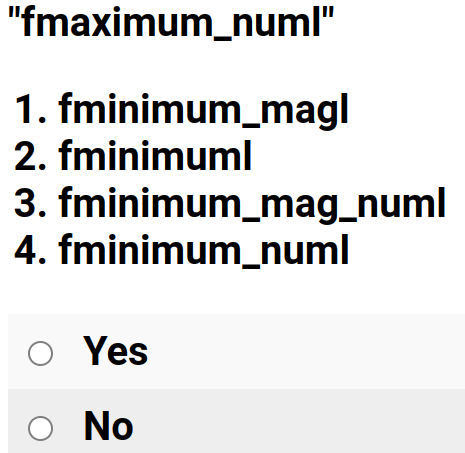
\includegraphics[scale=0.3]{abb/survey-example-positive.png}
    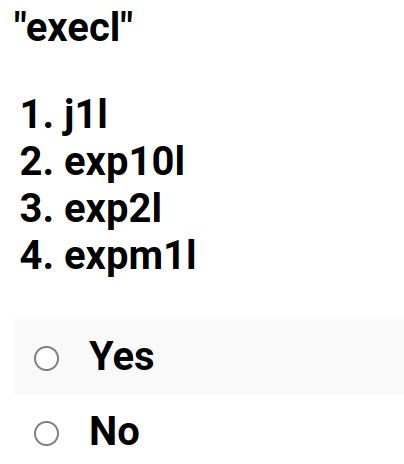
\includegraphics[scale=0.3]{abb/survey-example-negative.png}
  \end{center}
  \caption{
    Auf der linken Seite eine Frage aus dem Fragebogen die positiv
    beatwortet wurde und rechts eine Frage die negativ
    beatwortet wurde.
  }
\end{figure}
Die Auswertungsstrategie ist, dass jede Instanz einer Frage, die positiv
beantwortet wurde, einen Punkt gibt. Um einen Score für jede Strategie
zu berechnen, werden die Punkte summiert und dann anschließend durch die
$k$ zu erreichenden Punkte geteilt. Das Resultat ist ein normalisierter 
Score, der bei $\verb|score| = 1$ impliziert, dass alle Fragen positiv 
beantwortet wurden und bei $\verb|score| = 0$ impliziert, dass keine 
Frage positiv beantwortet wurde. Diese Auswertungsstrategie liefert 
folgendes Resultat:
\begin{center}
  \begin{tabular}{ |p{1.3cm}||p{3.8cm}|p{3cm}|p{1.8cm}|p{4.5cm}|  }
  \hline
  \multicolumn{5}{|c|}{Ergebnisse der Expertenbefragung} \\
  \hline
  Strategie & Funktionskommentare &  Funktionsnamen & \textit{Code2Vec} & Code-Llama-Erklärungen\\
  \hline
  Score   &  0                    &        0        &   0               & 0\\
  \hline
  \end{tabular}
\end{center} 
\hfill\\
Die Strategie mit dem höchsten Score ist demnach die, die Code-Llama-Erklärungen
verwendet hat. Da nun die beste Strategie identifiziert ist, 
werden im Folgenden die anderen Strategien mit dieser quantitativ verglichen.
% Diskussion der Ergebnisse
% Folgerungen das CodeLlamma "gute" Embeddings produziert 
\subsection{Quantitative Evaluierung} 
Im Folgenden wird eine Formel vorgestellt die zwei Datenmengen
auf Ähnlichket untersuchen soll. Dabei ist Ähnlichkeit hier,
ähnliche Nachbarschaftsbeziehungen zu besitzten. Im Folgenden
wird eine Datenmenge als Matrix 
$\mathbf{D} \in \mathbb{R}^{N\times l}$ beschrieben. Dabei 
ist $l \in \mathbb{N}$ die Dimension eines Datenpunkts und
$N \in \mathbb{N}$ die Anzahl der Datenpunkte. Folglich
besitzt jeder Datenpunkt $x \in \mathbb{R}^l$ einen eindeutigen
Index und zwar die $j$-te Zeile, für die gilt: $x = \mathbf{D}_j$, 
wobei $\mathbf{D}_j$ der $j$-te Zeilenvektor von $\mathbf{D}$ ist.\\
Zunächst wird eine Methode benötigt um Nachbarn von einen gegebenen
Punkt zu erlangen, dafür wird hier der 
\textit{K-Nearest-Neighbor-Algorithmus} verwendet. Dieser
gibt bei gegebenen Punkt die $k$ nächsten Nachbarn zurück. 
Also eine Funktion mit der Signatur: 
$NN_k: \mathbb{R}^{N\times l} \times \mathbb{R}^{l} \to \mathbb{N}^k$. 
Das heißt es die gesamte Datenmenge und ein Datenpunkt aus der Menge
eingeben und der Output ist ein Vektor aus indizes.
Der Output-Vektor enthält die indezes der nächsten Nachbarn. Diese sind 
aufsteigend sotiert, nach dem euklidischen Abstand von dem eingegeben
Punkt. Nun ist es möglich ein Nachbarschaftsverhältnis von einem Punkt
und seiner $k$ Nachbarn zu erhalten, in der Form des Vektors 
$v \in \mathbb{N}^k$.\\
Als nächstes wird eine Methode benötigt zwei 
Nachbarschaftsverhältnisse in der Form von 
zwei vektoren $u,v \in \mathbb{N}^k$ zu
vergleichen. Hierfür wird folgende Formel
verwendet:

\[
    \verb|compare|(u,v)_k = 
      \frac{1}{G_k} \sum^{k}_{i=1} 
      \frac{ \text{score}_{k}(u_i,i,v)}{log_2(i+1)}
\]
mit
\[
  \text{score}_k(x,i,v) = \begin{cases*} 
      1 & , $\exists j \in \mathbf{N}: x = v_j \land i = j$   \\
      \frac{1}{2} & , $\exists j \in \mathbf{N}: x = v_j \land i \neq j$\\
      0   & , \text{otherwise}
    \end{cases*}  \text{  und  }
    G_k := \sum_{i=1}^{k} \frac{1}{log_2(i+1)}.
\]


\begin{tikzpicture}
\begin{axis}[
    xlabel=$k$,
    ylabel=$\text{CMP}(A{,}B{,}k)$,
    width=0.8\textwidth, 
    height=0.6\textwidth
]

\addplot[green, thick] table
  {abb/summary-embeddings-high-comment-embeddings-high-non-empty-compare.dat};
\addplot[black, thick]
  table {abb/random-compare-plot-487x384.dat};
\addplot[blue, thick] 
  table {abb/summary-embeddings-high-name-embeddings-high-compare487.dat};
\addplot[red, thick] 
  table {abb/summary-embeddings-high-glibc-code2vec-high-compare487.dat};

\legend{
  Funktionskommentare und Code-Llama-Erklärungen,
  Zufällige Punkte und Code-Llama-Erklärungen,
  Funktiosnamen und Code-Llama-Erklärungen,
  \textit{Code2Vec} und Code-Llama-Erklärungen
}
\end{axis}
\end{tikzpicture}
% Formel um zwei Embedding spaces zu vergleichen
% Formel erklären und rechtfertigen
% Aus Umfrage rechtfertigen Codellama Summaries als gute
% embeddings zu verwenden
\subsection{Qualitative Evaluierung} 
%  \textit{t-SNE} Plots
% Vielleicht nochmal subsections mit Funktionsname, Funktionskommentare, 
% Funktionserklärung, und \textit{Code2Vec} Vektoren
% Probleme des jeweiligen Ansatzes mit drei Vektoren
\section{Diskussion}

In dem Beispiel ist gut zu erkennen, was in diesen Kontext mit semantischer
Ähnlichkeit gemeint ist. In dem positiven Besipiel, ist eine Funktion gegeben
die das Maximum zweier Fließkommazahlen berechnet und die vier
nächsten Nachbarn sind jeweils Variationen von Funktionen die das
Minimum von zwei fließkommazahlen berechnen. Diese Funktionen sind
semantisch ähnlich, da sie fast äquivalente Funktionen aus dem
Mathematikmodul sind. Im negativ Beispiel kreirt die 
gegebene Funktionen einen neuen Prozess, dagegen haben die nächsten
Nachbarn zwar einen sehr ähnlichen Namen, aber es sidn wieder Funktionen
aus dem Mathematikmodul.\\
%copy Evaluation
% Zusammenfassung der jeweiligen Resultate
% Funktionnamen -> Nicht geignet, da zu wenig informationen und abkürzungen
% Funktionskommentare -> Je nach Projekt geignet, aber nicht allgemeingültig
%     deswegen eher ungeignet
% \textit{Code2Vec} -> Kommt nur knapp an mit benutzuten Daten an Names ran also nicht 
% geignet
\section{Fazit}

Results: Comparing natural language supervised methods for creating Rich Binary Labels
\begin{itemize}
  \item Stabilität von Sentence Transformer
  \item Kommentare von Funktionen um Embeddings zu generieren
  \item Funktionsnamen von Funktionen um Embeddings zu generieren
  \item \textit{Code2Vec} um Embeddings zu generieren
  \item CodeLlama Erklärungen von Funktionen um Embeddings zu generieren
  \item Evaluierung durch tSNE-Plots
  \item Evaluierung durch Experten
  \item Evaluierung durch Formel
\end{itemize}
$ I_{k}: \mathbf{N} \times \mathbf{N} \times \mathbf{N}^{k} \to [0,1]$
\[ I_{k}(x,i,v) = \begin{cases*} 
1 & , $\exists j \in \mathbf{N}: x = v_j \land i = j$   \\
      \frac{1}{2} & , $\exists j \in \mathbf{N}: x = v_j \land i \neq j$\\
      0   & , \text{otherwise}
                \end{cases*} \]
$E_k: \nat^k \times \nat^k \to [0,1]$
\[ E_k(u,v) = \frac{1}{G_k} \sum^{k}_{i=1} \frac{I_k(u_i,i,v_i)}{log_2(i+1)}\]
wo $G_k := \sum_{i=1}^{k} \frac{1}{log_2(i+1)}$.\\
$CMP_k: \mathbf{R}^{N\times l} \times \mathbf{R}^{N\times l} \times 
\{ \mathbf{R}^l \times \mathbf{R}^{N\times l} \to \mathbf{N}^k \} 
\times \{ \mathcal{P}([0,1]) \to [0,1] \} \to [0,1]$

\[ CMP_k(X,Y,f_k,agg) = agg(\{E_k(f_k(X_j,X),f_k(Y_j,Y)) | j \in \{1,2,3, \dots N\}\})\]

\pagebreak

\addcontentsline{toc}{section}{Literatur}
\pagestyle{fancy}

\bibliographystyle{IEEEtran}
\bibliography{bibliography} %bib-filename
%\printglossary

\nocite{*} %List all bib-entries

\end{document}
